% Options for packages loaded elsewhere
\PassOptionsToPackage{unicode}{hyperref}
\PassOptionsToPackage{hyphens}{url}
\PassOptionsToPackage{dvipsnames,svgnames,x11names,table}{xcolor}
%
\documentclass[
  ignorenonframetext,
  aspectratio=169,
]{beamer}
\usepackage{pgfpages}
\setbeamertemplate{caption}[numbered]
\setbeamertemplate{caption label separator}{: }
\setbeamercolor{caption name}{fg=normal text.fg}
\beamertemplatenavigationsymbolsempty
% Prevent slide breaks in the middle of a paragraph
\widowpenalties 1 10000
\raggedbottom
\setbeamertemplate{part page}{
  \centering
  \begin{beamercolorbox}[sep=16pt,center]{part title}
    \usebeamerfont{part title}\insertpart\par
  \end{beamercolorbox}
}
\setbeamertemplate{section page}{
  \centering
  \begin{beamercolorbox}[sep=12pt,center]{part title}
    \usebeamerfont{section title}\insertsection\par
  \end{beamercolorbox}
}
\setbeamertemplate{subsection page}{
  \centering
  \begin{beamercolorbox}[sep=8pt,center]{part title}
    \usebeamerfont{subsection title}\insertsubsection\par
  \end{beamercolorbox}
}
\AtBeginPart{
  \frame{\partpage}
}
\AtBeginSection{
  \ifbibliography
  \else
    \frame{\sectionpage}
  \fi
}
\AtBeginSubsection{
  \frame{\subsectionpage}
}
\usepackage{amsmath,amssymb}
\usepackage{lmodern}
\usepackage{iftex}
\ifPDFTeX
  \usepackage[T1]{fontenc}
  \usepackage[utf8]{inputenc}
  \usepackage{textcomp} % provide euro and other symbols
\else % if luatex or xetex
  \usepackage{unicode-math}
  \defaultfontfeatures{Scale=MatchLowercase}
  \defaultfontfeatures[\rmfamily]{Ligatures=TeX,Scale=1}
  \setsansfont[]{Carlito}
  \setmonofont[]{DejaVuSansMono}
\fi
\usetheme[]{default}
\usefonttheme{professionalfonts}
\useinnertheme{rectangles}
\useoutertheme{number}
% Use upquote if available, for straight quotes in verbatim environments
\IfFileExists{upquote.sty}{\usepackage{upquote}}{}
\IfFileExists{microtype.sty}{% use microtype if available
  \usepackage[]{microtype}
  \UseMicrotypeSet[protrusion]{basicmath} % disable protrusion for tt fonts
}{}
\makeatletter
\@ifundefined{KOMAClassName}{% if non-KOMA class
  \IfFileExists{parskip.sty}{%
    \usepackage{parskip}
  }{% else
    \setlength{\parindent}{0pt}
    \setlength{\parskip}{6pt plus 2pt minus 1pt}}
}{% if KOMA class
  \KOMAoptions{parskip=half}}
\makeatother
\usepackage{xcolor}
\newif\ifbibliography
\usepackage{listings}
\newcommand{\passthrough}[1]{#1}
\lstset{defaultdialect=[5.3]Lua}
\lstset{defaultdialect=[x86masm]Assembler}
\usepackage{longtable,booktabs,array}
\usepackage{calc} % for calculating minipage widths
\usepackage{caption}
% Make caption package work with longtable
\makeatletter
\def\fnum@table{\tablename~\thetable}
\makeatother
\usepackage{graphicx}
\makeatletter
\def\maxwidth{\ifdim\Gin@nat@width>\linewidth\linewidth\else\Gin@nat@width\fi}
\def\maxheight{\ifdim\Gin@nat@height>\textheight\textheight\else\Gin@nat@height\fi}
\makeatother
% Scale images if necessary, so that they will not overflow the page
% margins by default, and it is still possible to overwrite the defaults
% using explicit options in \includegraphics[width, height, ...]{}
\setkeys{Gin}{width=\maxwidth,height=\maxheight,keepaspectratio}
% Set default figure placement to htbp
\makeatletter
\def\fps@figure{htbp}
\makeatother
\setlength{\emergencystretch}{3em} % prevent overfull lines
\providecommand{\tightlist}{%
  \setlength{\itemsep}{0pt}\setlength{\parskip}{0pt}}
\setcounter{secnumdepth}{-\maxdimen} % remove section numbering
\ifLuaTeX
\usepackage[bidi=basic]{babel}
\else
\usepackage[bidi=default]{babel}
\fi
\babelprovide[main,import]{american}
% get rid of language-specific shorthands (see #6817):
\let\LanguageShortHands\languageshorthands
\def\languageshorthands#1{}
\lstdefinelanguage{feenox}{
morekeywords={
      ABORT,
      ALIAS,
      AS,
      ASCENDING,
      ASCENDING_ORDER,
      ASCII_FILE,
      ASCII_FILE_PATH,
      AXISYMMETRIC,
      BC,
      BINARY_FILE,
      BINARY_FILE_PATH,
      BOUNDARY_CONDITION,
      CELL,
      CELLS,
      CLOSE,
      COLS,
      COLUMNS,
      DATA,
      DEFAULT_ARGUMENT_VALUE,
      DESCENDING,
      DESCENDING_ORDER,
      DIM,
      DIMENSION,
      DIMENSIONS,
      DIRICHLET_SCALING,
      DUMP,
      EIGEN_FORMULATION,
      EIGEN_SOLVER,
      ELSE,
      ENDIF,
      EPS,
      EPSABS,
      EPSREL,
      EPS_TYPE,
      FILE,
      FILE_FORMAT,
      FILE_PATH,
      FIND_EXTREMA,
      FIT,
      FORMAT,
      FROM,
      FUNCTION,
      FUNCTION_DATA,
      GAUSS,
      GRADIENT,
      GUESS,
      HEADER,
      HISTORY,
      ID,
      IF,
      IGNORE_NULL,
      I_MAX,
      I_MIN,
      IMPLICIT,
      INCLUDE,
      INITIAL_CONDITIONS,
      INITIAL_CONDITIONS_MODE,
      INPUT,
      INPUT_FILE,
      INTEGRATE,
      INTEGRATION,
      INTERPOLATION,
      INTERPOLATION_THRESHOLD,
      IS,
      K,
      K_bc,
      KSP,
      KSP_TYPE,
      LINEAR,
      LINEAR_SOLVER,
      M,
      MAIN,
      MATERIAL,
      MATRIX,
      MAX,
      MAX_ITER,
      M_bc,
      MESH,
      METHOD,
      MIN,
      MODE,
      MODES,
      MOMENT,
      NODE,
      NODES,
      NO_MESH,
      NOMESH,
      NONEWLINE,
      NON_LINEAR,
      NON_LINEAR_SOLVER,
      NONLINEAR_SOLVER,
      NO_PHYSICAL_NAMES,
      NSTEPS,
      OFFSET,
      OPEN,
      OUTPUT,
      OUTPUT_FILE,
      OVER,
      PATH,
      PC,
      PC_TYPE,
      PHASE_SPACE,
      PHYSICAL_ENTITY,
      PHYSICAL_GROUP,
      PRECONDITIONER,
      PRINT,
      PRINT_FUNCTION,
      PRINT_VECTOR,
      PROBLEM,
      PROGRESS,
      PROGRESS_ASCII,
      QUASISTATIC,
      RANGE_MAX,
      RANGE_MIN,
      REACTION,
      READ,
      READ_FIELD,
      READ_FUNCTION,
      READ_MESH,
      READ_VECTOR,
      RE_READ,
      RESIDUALS,
      RESULT,
      ROWS,
      SCALAR_FORMAT,
      SCALE,
      SEM,
      SEMAPHORE,
      SEP,
      SEPARATOR,
      SHEPARD_EXPONENT,
      SHEPARD_RADIUS,
      SHM,
      SHM_OBJECT,
      SIZE,
      SIZES,
      SNES,
      SNES_TYPE,
      SOLVE,
      SOLVE_PROBLEM,
      SORT_VECTOR,
      SPECTRAL_TRANSFORMATION,
      ST,
      STEP,
      STRING,
      ST_TYPE,
      TEXT,
      TIME_ADAPTATION,
      TIME_PATH,
      TO,
      TOL_ABS,
      TOL_REL,
      TRANSIENT,
      TRANSIENT_SOLVER,
      TS,
      TS_ADAPT,
      TS_ADAPT_TYPE,
      TS_TYPE,
      UNKNOWNS,
      UPDATE_EACH_STEP,
      VAR,
      VARIABLE,
      VARIABLES,
      VARS,
      VECTOR,
      VECTORS,
      VECTOR_SORT,
      VERBOSE,
      VIA,
      WRITE,
      WRITE_MESH,
      X0,
      X_INCREASES_FIRST,
      X_MAX,
      X_MIN,
      Y0,
      Y_MAX,
      Y_MIN,
      Z0,
      Z_MAX,
      Z_MIN,
      ALLOWED,
      AS_PROVIDED,
      NONE,
      POST,
      SKIP_HEADER_STEP,
      SKIP_STATIC_STEP,
      SKIP_STEP,
      SKIP_TIME,
      WAIT,
},
morekeywords={[2]
},
morekeywords={[3]
      dae_rtol,
      dae_rtol_0,
      done,
      done_0,
      done_static,
      done_static_0,
      done_transient,
      done_transient_0,
      dont_quit,
      dont_quit_0,
      dont_report,
      dont_report_0,
      dt,
      dt_0,
      end_time,
      end_time_0,
      i,
      i_0,
      infinite,
      infinite_0,
      in_static,
      in_static_0,
      in_static_first,
      in_static_first_0,
      in_static_last,
      in_static_last_0,
      in_transient,
      in_transient_0,
      in_transient_first,
      in_transient_first_0,
      in_transient_last,
      in_transient_last_0,
      j,
      j_0,
      max_dt,
      max_dt_0,
      min_dt,
      min_dt_0,
      ncores,
      ncores_0,
      on_gsl_error,
      on_gsl_error_0,
      on_nan,
      on_nan_0,
      on_sundials_error,
      on_sundials_error_0,
      pi,
      pi_0,
      pid,
      pid_0,
      quit,
      quit_0,
      realtime_scale,
      realtime_scale_0,
      report,
      report_0,
      static_steps,
      static_steps_0,
      step_static,
      step_static_0,
      step_transient,
      step_transient_0,
      t,
      t_0,
      zero,
      zero_0,
},
morekeywords={[4]
      abs,
      acos,
      asin,
      atan,
      atan2,
      ceil,
      clock,
      cos,
      cosh,
      cpu_time,
      d_dt,
      deadband,
      derivative,
      equal,
      exp,
      expint1,
      expint2,
      expint3,
      expintn,
      floor,
      func_min,
      gauss_kronrod,
      gauss_legendre,
      heaviside,
      if,
      integral,
      integral_dt,
      integral_euler_dt,
      is_even,
      is_in_interval,
      is_odd,
      j0,
      lag,
      lag_bilinear,
      lag_euler,
      last,
      limit,
      limit_dt,
      log,
      mark_max,
      mark_min,
      max,
      memory,
      min,
      mod,
      not,
      prod,
      quasi_random,
      random,
      random_gauss,
      root,
      round,
      sawtooth_wave,
      sgn,
      sin,
      sinh,
      sqrt,
      square_wave,
      sum,
      tan,
      tanh,
      threshold_max,
      threshold_min,
      triangular_wave,
      vecdot,
      vecmax,
      vecmaxindex,
      vecmin,
      vecminindex,
      vecnorm,
      vecsize,
      vecsum,
      wall_time,
},
sensitive=true,
morecomment=[l]{\#},
morestring=[b]\",
}
\definecolor{was_keyword1}{rgb}{0.0,0.0,0.4}
\definecolor{was_keyword2}{rgb}{0.0,0.2,0.0}
\definecolor{was_variable}{rgb}{0.5,0.2,0.2}
\definecolor{was_function}{rgb}{0.2,0.5,0.2}
\definecolor{was_comment}{rgb}{0.5,0.5,0.5}

\definecolor{bash_keyword1}{rgb}{0.2,0.2,0.2}
\definecolor{bash_keyword2}{rgb}{0.7,0.7,0.7}
\definecolor{bash_comment}{rgb}{0.5,0.5,0.5}

\definecolor{python_keyword2}{rgb}{0.5,0.2,0.8}

\definecolor{was_fondo}{rgb}{0.95,0.95,0.90}
\definecolor{fino_fondo}{rgb}{0.90,0.95,0.90}
\definecolor{gmsh_fondo}{rgb}{0.90,0.90,0.95}
\definecolor{terminal_fondo}{rgb}{0.2,0.2,0.2}
\definecolor{awk_fondo}{rgb}{0.95,0.90,0.95}
\definecolor{bash_fondo}{rgb}{0.90,0.90,0.90}

\definecolor{terminal_fore}{rgb}{1.0,1.0,1.0}


\newcommand{\MyHookSign}{\hbox{\ensuremath{\hookleftarrow}}}

% default
\lstset{
  basicstyle=\ttfamily\footnotesize,
  backgroundcolor=\color{bash_fondo},
  breaklines=true,
  prebreak={\space\MyHookSign},
  xleftmargin=0.2cm,
  xrightmargin=0.2cm,
  framesep=0.2cm,
  frame=single,
}


\lstdefinestyle{feenox}{
  language=feenox,
  basicstyle=\ttfamily\tiny,
  commentstyle={\color{was_comment}\normalfont\textit},
  keywordstyle=[1]{\color{was_keyword1}\ttfamily\textbf},
  keywordstyle=[2]{\color{was_keyword2}\ttfamily\textbf},
  keywordstyle=[3]{\color{was_variable}\textit},
  keywordstyle=[4]{\color{was_function}\textbf},
  backgroundcolor=\color{was_fondo},
  showstringspaces=true,
  breaklines=true,
  breakatwhitespace=true,
  prebreak={\space\MyHookSign},
  lineskip=-1pt,
  captionpos=b,
%   numbers=left,
%   stepnumber=5,
  xleftmargin=0.1cm,
  xrightmargin=0.1cm,
  framesep=0.1cm,
  frame=single,
}


\lstdefinestyle{bash}{
  language=bash,
  basicstyle=\ttfamily\tiny,
  commentstyle={\color{bash_comment}\normalfont\textit},
  keywordstyle=[1]{\color{bash_keyword1}\ttfamily\textbf},
  keywordstyle=[2]{\color{bash_keyword2}\ttfamily\textbf},
  backgroundcolor=\color{bash_fondo},
  showstringspaces=true,
  breaklines=true,
  breakatwhitespace=true,
  prebreak={\space\MyHookSign},
  lineskip=-1pt,
  captionpos=b,
%   numbers=left,
%   stepnumber=5,
  xleftmargin=0.1cm,
  xrightmargin=0.1cm,
  framesep=0.1cm,
  frame=single,
}


\lstdefinestyle{python}{
  language=python,
  basicstyle=\ttfamily\tiny,
  commentstyle={\color{bash_comment}\normalfont\textit},
  keywordstyle=[1]{\color{bash_keyword1}\ttfamily\textbf},
  keywordstyle=[2]{\color{python_keyword2}\ttfamily\textbf},
  backgroundcolor=\color{awk_fondo},
  showstringspaces=true,
  breaklines=true,
  breakatwhitespace=true,
  prebreak={\space\MyHookSign},
  lineskip=-1pt,
  captionpos=b,
%   numbers=left,
%   stepnumber=5,
  xleftmargin=0.1cm,
  xrightmargin=0.1cm,
  framesep=0.1cm,
  frame=single,
}


\lstdefinestyle{terminal}{
  language=,
  basicstyle=\ttfamily\tiny\color{terminal_fore},
  backgroundcolor=\color{terminal_fondo},
  breaklines=true,
  prebreak={\space\MyHookSign},
  xleftmargin=0.1cm,
  xrightmargin=0.1cm,
  framesep=0.1cm,
  frame=single,
}

\lstdefinestyle{c}{
  language=C,
  basicstyle=\ttfamily\tiny,
  commentstyle={\color{was_comment}\normalfont\textit},     
  keywordstyle=[1]{\color{was_keyword1}\ttfamily\textbf},   
  keywordstyle=[2]{\color{was_keyword2}\ttfamily\textbf},   
  keywordstyle=[3]{\color{was_variable}\textit},            
  keywordstyle=[4]{\color{was_function}\textbf},            
  backgroundcolor=\color{gmsh_fondo},                       
  showstringspaces=true,                                    
  breaklines=true,                                          
  breakatwhitespace=true,                                   
  prebreak={\space\MyHookSign},                             
  lineskip=-1pt,                                            
  captionpos=b,
%   numbers=left,
%   stepnumber=5,
  xleftmargin=0.1cm,                                        
  xrightmargin=0.1cm,                                       
  framesep=0.1cm,                                           
  frame=single,                                             
}

\lstdefinestyle{cpp}{
  language=C++,
  basicstyle=\ttfamily\footnotesize,                                
  commentstyle={\color{was_comment}\normalfont\textit},     
  keywordstyle=[1]{\color{was_keyword1}\ttfamily\textbf},   
  keywordstyle=[2]{\color{was_keyword2}\ttfamily\textbf},   
  keywordstyle=[3]{\color{was_variable}\textit},            
  keywordstyle=[4]{\color{was_function}\textbf},            
  backgroundcolor=\color{gmsh_fondo},                       
  showstringspaces=true,                                    
  breaklines=true,                                          
  breakatwhitespace=true,                                   
  prebreak={\space\MyHookSign},                             
  lineskip=-1pt,                                            
  captionpos=b,
%   numbers=left,
%   stepnumber=5,
  xleftmargin=0.2cm,                                        
  xrightmargin=0.4cm,                                       
  framesep=0.1cm,                                           
  frame=single,                                             
}




\lstdefinestyle{awk}{
  language=awk,
  basicstyle=\ttfamily\footnotesize,                                
  commentstyle={\color{was_comment}\normalfont\textit},     
  keywordstyle=[1]{\color{was_keyword1}\ttfamily\textbf},   
  keywordstyle=[2]{\color{was_keyword2}\ttfamily\textbf},   
  keywordstyle=[3]{\color{was_variable}\textit},            
  keywordstyle=[4]{\color{was_function}\textbf},            
  backgroundcolor=\color{awk_fondo},                       
  showstringspaces=true,                                    
  breaklines=true,                                          
  breakatwhitespace=true,                                   
  prebreak={\space\MyHookSign},                             
  lineskip=-1pt,                                            
  captionpos=b,
%   numbers=left,
%   stepnumber=5,
  xleftmargin=0.2cm,                                        
  xrightmargin=0.4cm,                                       
  framesep=0.1cm,                                           
  frame=single,                                             
}



\ifLuaTeX
  \usepackage{selnolig}  % disable illegal ligatures
\fi
\IfFileExists{bookmark.sty}{\usepackage{bookmark}}{\usepackage{hyperref}}
\IfFileExists{xurl.sty}{\usepackage{xurl}}{} % add URL line breaks if available
\urlstyle{same} % disable monospaced font for URLs
\hypersetup{
  pdftitle={FeenoX, a cloud-first free and open source finite-element(ish) tool},
  pdfauthor={Jeremy Theler},
  pdflang={en-US},
  colorlinks=true,
  linkcolor={Maroon},
  filecolor={Maroon},
  citecolor={Blue},
  urlcolor={Blue},
  pdfcreator={LaTeX via pandoc}}

\title{FeenoX, a cloud-first free and open source finite-element(ish)
tool}
\author{Jeremy Theler}
\date{8499f36---2022-10-23+}

\begin{document}
\frame{\titlepage}

\begin{frame}{}
\protect\hypertarget{section}{}
\begin{columns}[T]
\begin{column}{0.6\textwidth}
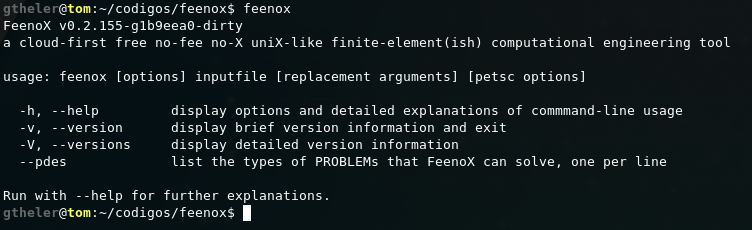
\includegraphics{feenox-console.png}

\begin{itemize}
\tightlist
\item
  The last X makes it rhyme with Unix and Linux.
\item
  ``noX'' means that there is no graphical (i.e.~X) interface
\item
  Fee-no means that there are no fees involved (free as in ``free
  beer'')
\item
  FeenoX is the successor of the now-superseded FEA program Fino
\item
  With some luck one can read nite ElEments NO-X''
\item
  With mode luck, ``FrEE'' (as in ``free speech'')
\end{itemize}
\end{column}

\begin{column}{0.4\textwidth}
\begin{itemize}
\tightlist
\item
  cloud-first (\(\neq\) cloud-friendly)

  \begin{itemize}
  \tightlist
  \item
    cloud \(=\) somebody else's computer(s)
  \end{itemize}
\item
  free \& open source (\(\neq\) gratis)

  \begin{itemize}
  \tightlist
  \item
    free \(\simeq\) open source
  \item
    it is not about \textbf{price}!
  \item
    free is about \textbf{freedom}
  \item
    open is about \textbf{transparency}
  \end{itemize}
\item
  finite-element(ish)

  \begin{itemize}
  \tightlist
  \item
    PDEs with FEM \& FVM
  \item
    ODEs with IMEX
  \item
    generic math problems
  \end{itemize}
\item
  computational engineering tool

  \begin{itemize}
  \tightlist
  \item
    the right tool for the right problem, right?
  \end{itemize}
\end{itemize}
\end{column}
\end{columns}
\end{frame}

\begin{frame}{How do we write papers/reports/documents?}
\protect\hypertarget{how-do-we-write-papersreportsdocuments}{}
\newcommand{\todonow}{\textcolor{Plum}{TO-DO}}
\newcommand{\todolater}{\textcolor{Orange}{TO-DO}}
\newcommand{\good}{\textcolor{OliveGreen}{$\checkmark$}}
\newcommand{\bad}{\textcolor{red}{$\times$}}
\newcommand{\neutral}{\textcolor{DarkBlue}{$\sim$}}

\begin{columns}[T]
\begin{column}{0.25\textwidth}
\centering \onslide<1->{
\includegraphics[height=2cm]{word}}
\end{column}

\begin{column}{0.25\textwidth}
\centering \onslide<3->{
\includegraphics[height=2cm]{google_docs}}
\end{column}

\begin{column}{0.25\textwidth}
\centering \onslide<4->{
\includegraphics[height=2cm]{markdown}}
\end{column}

\begin{column}{0.25\textwidth}
\centering \onslide<2->{
\includegraphics[height=2cm]{tex}}
\end{column}
\end{columns}

\rowcolors{1}{black!10}{black!0}

\begin{longtable}[]{@{}
  >{\raggedright\arraybackslash}p{(\columnwidth - 8\tabcolsep) * \real{0.1791}}
  >{\centering\arraybackslash}p{(\columnwidth - 8\tabcolsep) * \real{0.1791}}
  >{\centering\arraybackslash}p{(\columnwidth - 8\tabcolsep) * \real{0.1940}}
  >{\centering\arraybackslash}p{(\columnwidth - 8\tabcolsep) * \real{0.2537}}
  >{\centering\arraybackslash}p{(\columnwidth - 8\tabcolsep) * \real{0.1940}}@{}}
\toprule()
\begin{minipage}[b]{\linewidth}\raggedright
Feature
\end{minipage} & \begin{minipage}[b]{\linewidth}\centering
\onslide<1->{Word}
\end{minipage} & \begin{minipage}[b]{\linewidth}\centering
\onslide<3->{Docs}
\end{minipage} & \begin{minipage}[b]{\linewidth}\centering
\onslide<4->{Markdown$^{*}$}
\end{minipage} & \begin{minipage}[b]{\linewidth}\centering
\onslide<2->{\TeX}
\end{minipage} \\
\midrule()
\endhead
Aesthetics & \onslide<1->{\textcolor{red}{$\times$}} &
\onslide<3->{\textcolor{red}{$\times$}} &
\onslide<4->{\textcolor{OliveGreen}{$\checkmark$}} &
\onslide<2->{\textcolor{OliveGreen}{$\checkmark$}} \\
Convertibility & \onslide<1->{\textcolor{DarkBlue}{$\sim$}} &
\onslide<3->{\textcolor{DarkBlue}{$\sim$}} &
\onslide<4->{\textcolor{OliveGreen}{$\checkmark$}} &
\onslide<2->{\textcolor{DarkBlue}{$\sim$}} \\
Traceability & \onslide<1->{\textcolor{red}{$\times$}} &
\onslide<3->{\textcolor{DarkBlue}{$\sim$}} &
\onslide<4->{\textcolor{OliveGreen}{$\checkmark$}} &
\onslide<2->{\textcolor{OliveGreen}{$\checkmark$}} \\
Mobile-friendliness & \onslide<1->{\textcolor{red}{$\times$}} &
\onslide<3->{\textcolor{OliveGreen}{$\checkmark$}} &
\onslide<4->{\textcolor{OliveGreen}{$\checkmark$}} &
\onslide<2->{\textcolor{red}{$\times$}} \\
Collaborative & \onslide<1->{\textcolor{red}{$\times$}} &
\onslide<3->{\textcolor{OliveGreen}{$\checkmark$}} &
\onslide<4->{\textcolor{OliveGreen}{$\checkmark$}} &
\onslide<2->{\textcolor{DarkBlue}{$\sim$}} \\
Openness & \onslide<1->{\textcolor{red}{$\times$}} &
\onslide<3->{\textcolor{red}{$\times$}} &
\onslide<4->{\textcolor{OliveGreen}{$\checkmark$}} &
\onslide<2->{\textcolor{OliveGreen}{$\checkmark$}} \\
Friendliness & \onslide<1->{\textcolor{OliveGreen}{$\checkmark$}} &
\onslide<3->{\textcolor{OliveGreen}{$\checkmark$}} &
\onslide<4->{\textcolor{DarkBlue}{$\sim$}} &
\onslide<2->{\textcolor{red}{$\times$}} \\
\bottomrule()
\end{longtable}

\onslide<4->{\centering $^*$ \href{https://en.wikipedia.org/wiki/Markdown}{Markdown} +
\href{https://pandoc.org/}{Pandoc} + \href{https://git-scm.com/}{Git} +
\href{https://github.com/}{Github} /
\href{https://about.gitlab.com/}{Gitlab} /
\href{https://gitea.com/}{Gitea}}
\end{frame}

\begin{frame}{How do we perform scientific/engineering computations?}
\protect\hypertarget{how-do-we-perform-scientificengineering-computations}{}
\begin{columns}[T]
\begin{column}{0.25\textwidth}
\centering \onslide<1->{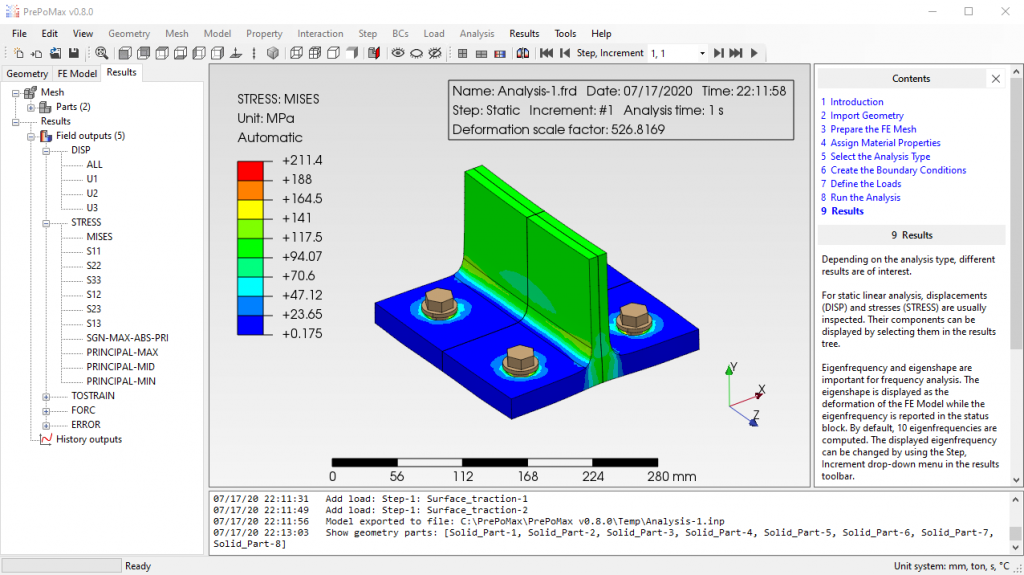
\includegraphics[height=2cm]{prepomax}}
\end{column}

\begin{column}{0.25\textwidth}
\centering \onslide<3->{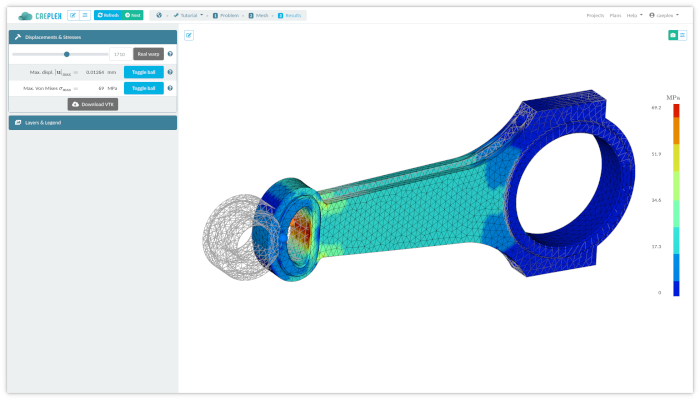
\includegraphics[height=2cm]{caeplex}}
\end{column}

\begin{column}{0.25\textwidth}
\centering \onslide<4->{
\includegraphics[height=2cm]{feenox-logo}}
\end{column}

\begin{column}{0.25\textwidth}
\centering \onslide<2->{
\includegraphics[height=2cm]{libraries}}
\end{column}
\end{columns}

\rowcolors{1}{black!10}{black!0}

\begin{longtable}[]{@{}
  >{\raggedright\arraybackslash}p{(\columnwidth - 8\tabcolsep) * \real{0.1600}}
  >{\centering\arraybackslash}p{(\columnwidth - 8\tabcolsep) * \real{0.2400}}
  >{\centering\arraybackslash}p{(\columnwidth - 8\tabcolsep) * \real{0.2067}}
  >{\centering\arraybackslash}p{(\columnwidth - 8\tabcolsep) * \real{0.1867}}
  >{\centering\arraybackslash}p{(\columnwidth - 8\tabcolsep) * \real{0.2067}}@{}}
\toprule()
\begin{minipage}[b]{\linewidth}\raggedright
Feature
\end{minipage} & \begin{minipage}[b]{\linewidth}\centering
\onslide<1->{Desktop GUIs}
\end{minipage} & \begin{minipage}[b]{\linewidth}\centering
\onslide<3->{Web frontends}
\end{minipage} & \begin{minipage}[b]{\linewidth}\centering
\onslide<4->{FeenoX$^{*}$}
\end{minipage} & \begin{minipage}[b]{\linewidth}\centering
\onslide<2->{Libraries}
\end{minipage} \\
\midrule()
\endhead
Flexibility & \onslide<1->{\textcolor{DarkBlue}{$\sim$}} &
\onslide<3->{\textcolor{red}{$\times$}} &
\onslide<4->{\textcolor{OliveGreen}{$\checkmark$}} &
\onslide<2->{\textcolor{OliveGreen}{$\checkmark$}} \\
Scalability & \onslide<1->{\textcolor{red}{$\times$}} &
\onslide<3->{\textcolor{DarkBlue}{$\sim$}} &
\onslide<4->{\textcolor{OliveGreen}{$\checkmark$}} &
\onslide<2->{\textcolor{OliveGreen}{$\checkmark$}} \\
Traceability & \onslide<1->{\textcolor{red}{$\times$}} &
\onslide<3->{\textcolor{DarkBlue}{$\sim$}} &
\onslide<4->{\textcolor{OliveGreen}{$\checkmark$}} &
\onslide<2->{\textcolor{OliveGreen}{$\checkmark$}} \\
Cloudlity & \onslide<1->{\textcolor{red}{$\times$}} &
\onslide<3->{\textcolor{OliveGreen}{$\checkmark$}} &
\onslide<4->{\textcolor{OliveGreen}{$\checkmark$}} &
\onslide<2->{\textcolor{OliveGreen}{$\checkmark$}} \\
Collaborative & \onslide<1->{\textcolor{red}{$\times$}} &
\onslide<3->{\textcolor{OliveGreen}{$\checkmark$}} &
\onslide<4->{\textcolor{DarkBlue}{$\sim$}} &
\onslide<2->{\textcolor{red}{$\times$}} \\
Openness &
\onslide<1->{\textcolor{OliveGreen}{$\checkmark$}/\textcolor{DarkBlue}{$\sim$}/\textcolor{red}{$\times$}}
& \onslide<3->{\textcolor{red}{$\times$}} &
\onslide<4->{\textcolor{OliveGreen}{$\checkmark$}} &
\onslide<2->{\textcolor{OliveGreen}{$\checkmark$}} \\
Friendliness & \onslide<1->{\textcolor{OliveGreen}{$\checkmark$}} &
\onslide<3->{\textcolor{OliveGreen}{$\checkmark$}} &
\onslide<4->{\textcolor{DarkBlue}{$\sim$}} &
\onslide<2->{\textcolor{red}{$\times$}} \\
\bottomrule()
\end{longtable}

\onslide<4->{\centering $^*$ \href{https://seamplex.com/feenox}{FeenoX} +
\href{http://gmsh.info}{Gmsh} + \href{https://www.paraview.org/}{Paraview} + \href{https://git-scm.com/}{Git} +
\href{https://github.com/}{Github} /
\href{https://about.gitlab.com/}{Gitlab} /
\href{https://gitea.com/}{Gitea}}
\end{frame}

\begin{frame}{Free \& open-source software in CAE}
\protect\hypertarget{free-open-source-software-in-cae}{}
\begin{columns}[T]
\begin{column}{0.5\textwidth}
\begin{itemize}
\item
  Free software

  \begin{itemize}
  \tightlist
  \item
    Ethical principles
  \item
    You are \textbf{free} to modify the code to make the computation you
    want/need
  \item
    You are \textbf{free} to hire somebody to modify it for you
  \end{itemize}
\end{itemize}
\end{column}
\end{columns}

\begin{column}{0.5\textwidth}
\begin{itemize}
\item
  Open source

  \begin{itemize}
  \tightlist
  \item
    Technical principles
  \item
    You \textbf{can} see what the code does and not have to rely on the
    documentation
  \item
    You \textbf{can} hire somebody to verify the code for you
  \end{itemize}
\end{itemize}
\end{column}

::::::::::::::
\end{frame}

\begin{frame}{Notes on FOSS in CAE}
\protect\hypertarget{notes-on-foss-in-cae}{}
\begin{itemize}
\tightlist
\item
  Free software \(\simeq\) Open source \(\neq\) ``source available,''
  e.g.

  \begin{itemize}
  \tightlist
  \item
    Serpent asks for an NDA to access the source
  \item
    CalculiX's source code is unintelligible
  \end{itemize}
\item
  It is \textbf{not} about money!
\item
  It is \textbf{not} about licenses!

  \begin{itemize}
  \tightlist
  \item
    Every piece of software has licenses---especially FOSS
  \end{itemize}
\end{itemize}
\end{frame}

\begin{frame}
\begin{itemize}
\tightlist
\item
  At the end of the day, FOSS may be more expensive than
  \emph{privative}

  \begin{itemize}
  \tightlist
  \item
    Do \textbf{not} say ``commercial'' as opposed to FOSS!
  \end{itemize}
\item
  But it is worth it in terms of

  \begin{itemize}
  \tightlist
  \item
    accuracy: you are allowed to see the equations
  \item
    flexibility: you are allowed to make it work like you want
  \end{itemize}
\end{itemize}
\end{frame}

\begin{frame}
\begin{itemize}
\tightlist
\item
  Remember: it is your signature that will appear on the engineering
  reports you create!
\end{itemize}
\end{frame}

\begin{frame}{Software Requirement Specifications}
\protect\hypertarget{software-requirement-specifications}{}
Let's assume there is a a fictitious \& imaginary ``Request for
Quotation'' for a computational tool:

\begin{columns}[T]
\begin{column}{0.35\textwidth}
\begin{enumerate}
\tightlist
\item
  Introduction

  \begin{itemize}
  \tightlist
  \item
    1.1. Objective
  \item
    1.2. Scope
  \end{itemize}
\item
  Architecture

  \begin{itemize}
  \tightlist
  \item
    2.1. Deployment
  \item
    2.2. Execution
  \item
    2.3. Efficiency
  \item
    2.4. Scalability
  \item
    2.5. Flexibility
  \item
    2.6. Extensibility
  \item
    2.7. Interoperability
  \end{itemize}
\end{enumerate}
\end{column}

\begin{column}{0.5\textwidth}
\begin{enumerate}
\setcounter{enumi}{2}
\tightlist
\item
  Interfaces

  \begin{itemize}
  \tightlist
  \item
    3.1. Problem input
  \item
    3.2. Results output
  \end{itemize}
\item
  Quality assurance

  \begin{itemize}
  \tightlist
  \item
    4.1. Reproducibility and traceability
  \item
    4.2. Automated testing
  \item
    4.3. Bug reporting and tracking
  \item
    4.4. Verification
  \item
    4.5. Validation
  \item
    4.6. Documentation
  \end{itemize}
\end{enumerate}
\end{column}
\end{columns}

\begin{exampleblock}{FeenoX Software Design Specifications}
\protect\hypertarget{feenox-software-design-specifications}{}
\begin{itemize}
\tightlist
\item
  A fictitious \& imaginary tender applying to the SRS addressing each
  section.
\end{itemize}
\end{exampleblock}
\end{frame}

\begin{frame}[fragile]{}
\protect\hypertarget{section-1}{}
\begin{columns}[T]
\begin{column}{0.5\textwidth}
\begin{block}{1. Introduction}
\protect\hypertarget{introduction}{}
\begin{itemize}
\tightlist
\item
  Application to industrial problems

  \begin{itemize}
  \tightlist
  \item
    Open source (to allow third-party V\&V)
  \end{itemize}
\item
  First version should handle some problems
\item
  Extensible to other problems \& formulations

  \begin{itemize}
  \tightlist
  \item
    Free (as in freedom to hire somebody to modify/extend it)
  \end{itemize}
\end{itemize}

\begin{block}{1.1. Objective}
\protect\hypertarget{objective}{}
\begin{itemize}
\tightlist
\item
  Solve DAEs and/or PDEs

  \begin{itemize}
  \tightlist
  \item
    Heat conduction
  \item
    Elasticity
  \item
    Electromagnetism
  \item
    Fluid mechanics
  \item
    \ldots{}
  \end{itemize}
\item
  State-of-the-art cloud-first
\end{itemize}
\end{block}
\end{block}
\end{column}

\pause

\begin{column}{0.5\textwidth}
\begin{exampleblock}{FeenoX}
\protect\hypertarget{feenox}{}
\begin{itemize}
\tightlist
\item
  Free as ``software libre''

  \begin{itemize}
  \tightlist
  \item
    GPLv3+
  \item
    Only FOSS dependencies
  \item
    Main target is \passthrough{\lstinline!linux-x86\_64!}
  \item
    Development environment is Debian \medskip
  \end{itemize}
\item
  Initial version supports

  \begin{itemize}
  \tightlist
  \item
    Dynamical systems (DAE)
  \item
    Laplace/Poisson/Helmholtz (FEM)
  \item
    Heat (FEM)
  \item
    Elasticity (FEM)
  \item
    Modal (FEM)
  \item
    Neutron transport and diffusion (FEM/FVM)
  \end{itemize}
\item
  Templates for more formulations

  \begin{itemize}
  \tightlist
  \item
    Electromagnetism
  \item
    Chemical diffusion/reaction
  \item
    Fluid mechanics?
  \end{itemize}
\end{itemize}
\end{exampleblock}
\end{column}
\end{columns}
\end{frame}

\begin{frame}[fragile]{}
\protect\hypertarget{section-2}{}
\begin{columns}[T]
\begin{column}{0.5\textwidth}
\begin{block}{1.2. Scope}
\protect\hypertarget{scope}{}
\begin{itemize}
\tightlist
\item
  The problem should be defined programatically

  \begin{itemize}
  \tightlist
  \item
    One or more input files (JSON, YAML, ad-hoc format), and/or
  \item
    An API for high-level language (Python, Julia, etc.)
  \end{itemize}
\item
  There is no need to \emph{include} a GUI

  \begin{itemize}
  \tightlist
  \item
    The tool should \emph{allow} a GUI to be used

    \begin{itemize}
    \tightlist
    \item
      Desktop
    \item
      Web
    \item
      Mobile
    \end{itemize}
  \end{itemize}
\item
  The mesh can be an input

  \begin{itemize}
  \tightlist
  \item
    As long as its creation meets the SRS
  \end{itemize}
\item
  Include documentation about how a\ldots{}

  \begin{itemize}
  \tightlist
  \item
    Pre-processor should create inputs
  \item
    Post-processor should read outputs
  \end{itemize}
\end{itemize}
\end{block}
\end{column}

\pause

\begin{column}{0.5\textwidth}
\begin{exampleblock}{FeenoX}
\protect\hypertarget{feenox-1}{}
\begin{itemize}
\tightlist
\item
  No GUI, console binary executable
\item
  ``Transfer-function''-like between I/O

  \begin{itemize}
  \item
    No need to recompile the binary

    
\includegraphics[width=0.9\textwidth,height=\textheight]{transfer.svg}~
  \end{itemize}
\item
  English-like syntactic-sugared input files

  \begin{itemize}
  \tightlist
  \item
    Nouns are definitions
  \item
    Verbs are instructions
  \end{itemize}
\item
  Python \& Julia API: \textcolor{Orange}{TO-DO}

  \begin{itemize}
  \tightlist
  \item
    But already taken into account in the design \& implementation
  \end{itemize}
\item
  Separate mesher

  \begin{itemize}
  \tightlist
  \item
    \href{http://gmsh.info/}{Gmsh} (GPLv2, meets SRS)
  \item
    Anything that writes \passthrough{\lstinline!.msh!}
  \end{itemize}
\item
  Possibility to use GUI

  \begin{itemize}
  \tightlist
  \item
    CAEplex \url{https://www.caeplex.com}
  \end{itemize}
\end{itemize}
\end{exampleblock}
\end{column}
\end{columns}
\end{frame}

\begin{frame}[fragile]{Transfer-function \& English-like input: Lorenz'
system}
\protect\hypertarget{transfer-function-english-like-input-lorenz-system}{}
\begin{columns}[T]
\begin{column}{0.45\textwidth}
Solve \[
\begin{cases}
\dot{x} = \sigma \cdot (y - x) \\
\dot{y} = x \cdot (r - z) - y \\
\dot{z} = x y - b z
\end{cases}
\]

\noindent for \(0 < t < 40\) with initial conditions

\[
\begin{cases}
x(0) = -11\\
y(0) = -16\\
z(0) = 22.5\\
\end{cases}
\]

\noindent and \(\sigma=10\), \(r=28\) and \(b=8/3\).
\end{column}

\pause

\begin{column}{0.55\textwidth}
\begin{lstlisting}[style=feenox]
PHASE_SPACE x y z
end_time = 40         # dimensionless time

sigma = 10            # parameters
r = 28
b = 8/3

x_0 = -11             # initial conditions
y_0 = -16
z_0 = 22.5

# Lorenz's equations as written in 1963
x_dot = sigma*(y - x)
y_dot = x*(r - z) - y
z_dot = x*y - b*z

PRINT %e t x y z      # four-column plain-ASCII output
\end{lstlisting}

\begin{lstlisting}[style=terminal]
$ feenox lorenz.fee
0.000000e+00    -1.100000e+01   -1.600000e+01   2.250000e+01
2.384186e-07    -1.100001e+01   -1.600001e+01   2.250003e+01
4.768372e-07    -1.100002e+01   -1.600002e+01   2.250006e+01
[...]
3.997567e+01    4.442995e+00    3.764391e+00    2.347301e+01
3.998290e+01    4.399950e+00    3.886609e+00    2.314602e+01
3.999012e+01    4.368713e+00    4.016860e+00    2.282821e+01
$
\end{lstlisting}
\end{column}
\end{columns}
\end{frame}

\begin{frame}{Lorenz' system}
\protect\hypertarget{lorenz-system}{}
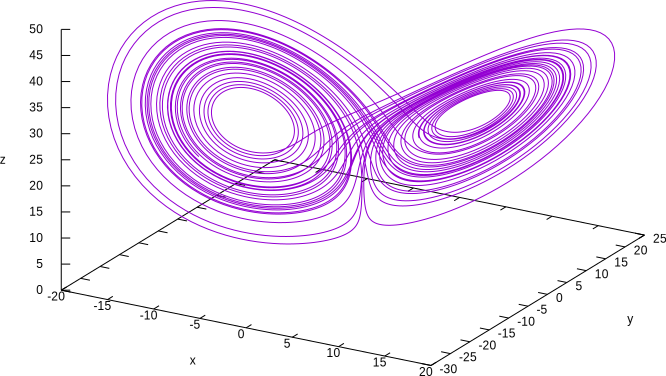
\includegraphics{lorenz.svg}
\end{frame}

\begin{frame}{Web interface: CAEplex, finite elements in the cloud}
\protect\hypertarget{web-interface-caeplex-finite-elements-in-the-cloud}{}
\centering 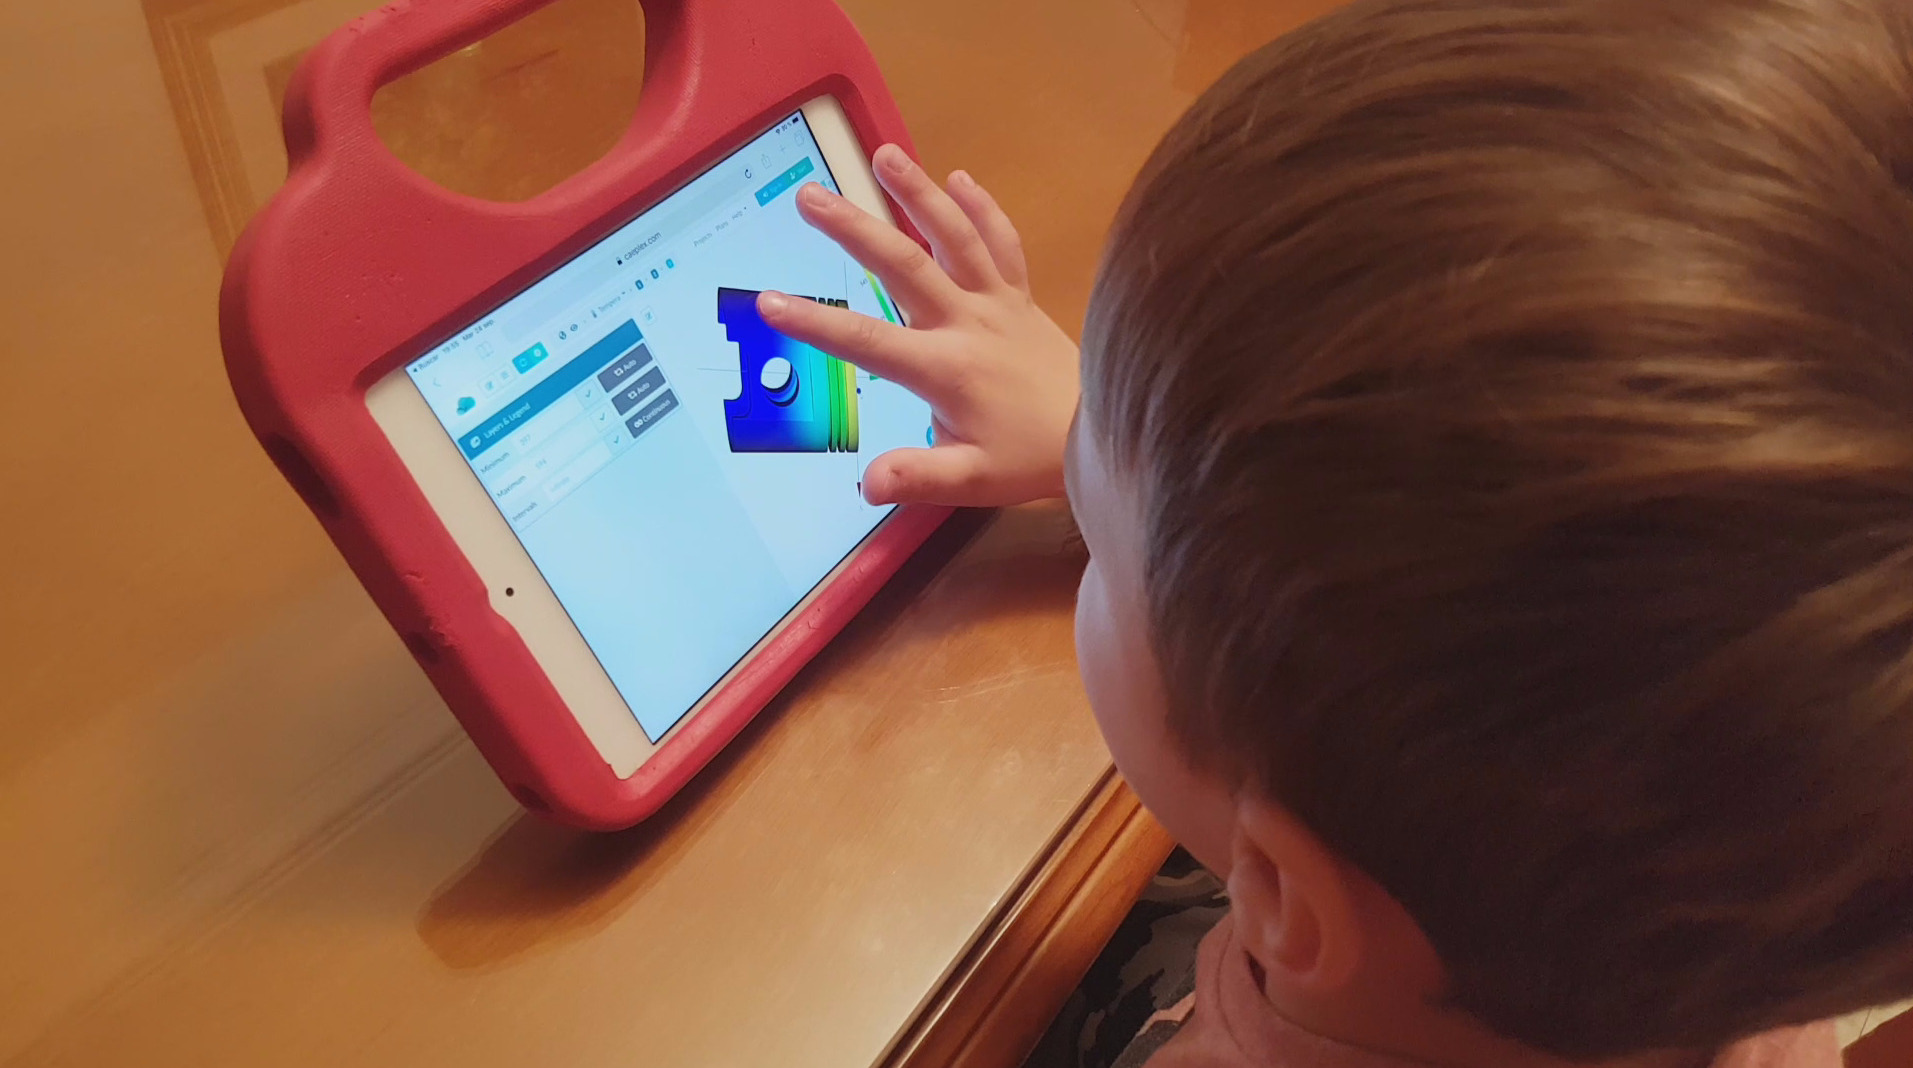
\includegraphics[width=0.7\textwidth,height=\textheight]{caeplex-ipad.jpg}

\url{https://www.seamplex.com/feenox/videos/caeplex-ipad.mp4}

\url{https://www.caeplex.com}
\end{frame}

\begin{frame}[fragile]{}
\protect\hypertarget{section-3}{}
\begin{columns}[T]
\begin{column}{0.5\textwidth}
\begin{block}{2. Architecture}
\protect\hypertarget{architecture}{}
\newcommand{\unix}{{\textcolor{cyan}{UNIX}}}
\newcommand{\ruleof}[1]{{\textcolor{cyan}{Rule of {#1}}}}
\newcommand{\ruleofpar}[1]{\vspace{-0.25cm}\hfill{\footnotesize\textcolor{cyan}{(Rule of {#1})}}}

\begin{itemize}
\tightlist
\item
  Should run on mainstream cloud servers

  \begin{itemize}
  \tightlist
  \item
    GNU/Linux
  \item
    Multi-core Intel-compatible CPUs
  \item
    Several levels of memory cache
  \item
    A few Gb of RAM
  \item
    Several Gb of SSD
  \item
    Either

    \begin{itemize}
    \tightlist
    \item
      Bare metal
    \item
      Virtualized
    \item
      Containerized
    \end{itemize}
  \end{itemize}
\item
  Standard compilers, libraries and dependencies

  \begin{itemize}
  \tightlist
  \item
    Available in common GNU/Linux repositories
  \item
    Preferable 100\% open source
  \item
    Adhere to well-established standards
  \end{itemize}
\end{itemize}
\end{block}
\end{column}

\pause

\begin{column}{0.5\textwidth}
\begin{exampleblock}{FeenoX}
\protect\hypertarget{feenox-2}{}
\begin{itemize}
\item
  Third-system effect (after v1 \& v2)
\item
  {\textcolor{cyan}{UNIX}} philosophy: ``do one thing well''

  \begin{itemize}
  \tightlist
  \item
    {\textcolor{cyan}{Rule of {separation}}}: no GUI
  \item
    {\textcolor{cyan}{Rule of {composition}}}: Gnuplot, Gmsh, \ldots{}
  \item
    \ldots more rules to come!
  \end{itemize}
\item
  Third-party math libraries

  \begin{itemize}
  \item
    GNU GSL, PETSc, SLEPc, SUNDIALS
  \item
    {\textcolor{cyan}{Rule of {modularity}}}
  \end{itemize}
\item
  Dependencies available in APT

\begin{lstlisting}[style=terminal]
apt-get install git gcc make automake autoconf
apt-get install libgsl-dev
apt-get install lib-sundials-dev petsc-dev slepc-dev
\end{lstlisting}
\item
  Sources on
  \href{https://github.com/seamplex/feenox}{github.com/seamplex/feenox}

\begin{lstlisting}[style=terminal]
git clone https://github.com/seamplex/feenox
\end{lstlisting}
\item
  Autotools \& friends for compilation

\begin{lstlisting}[style=terminal]
./autogen.sh && ./configure && make
\end{lstlisting}
\end{itemize}
\end{exampleblock}
\end{column}
\end{columns}
\end{frame}

\begin{frame}{}
\protect\hypertarget{section-4}{}
\begin{columns}[T]
\begin{column}{0.5\textwidth}
\begin{block}{2. Architecture}
\protect\hypertarget{architecture-1}{}
\begin{itemize}
\tightlist
\item
  Small coarse problems should be run in single hosts to check inputs

  \begin{itemize}
  \tightlist
  \item
    Local desktop/laptops (not needed but suggested)
  \item
    Windows and MacOS (not needed but suggested)
  \item
    Small cloud instances
  \end{itemize}
\item
  Large actual problems should be split into several hosts

  \begin{itemize}
  \tightlist
  \item
    HPC clusters
  \item
    Scalable cloud instances
  \end{itemize}
\item
  Mobile devices (not needed but suggested)

  \begin{itemize}
  \tightlist
  \item
    As control/monitoring devices
  \end{itemize}
\end{itemize}
\end{block}
\end{column}

\pause

\begin{column}{0.5\textwidth}
\begin{exampleblock}{FeenoX}
\protect\hypertarget{feenox-3}{}
\begin{itemize}
\item
  Tested on

  \begin{itemize}
  \tightlist
  \item
    Raspberry Pi
  \item
    Laptop (GNU/Linux \& Windows 10)
  \item
    Macbook
  \item
    Desktop PC
  \item
    Bare-metal servers
  \item
    Vagrant/Virtualbox
  \item
    Docker/Kubernetes
  \item
    AWS/DigitalOcean/Contabo
  \end{itemize}
\item
  Parallelization:

  \begin{itemize}
  \tightlist
  \item
    Gmsh partitioning with METIS
  \item
    PETSc/SLEPc with MPI
  \end{itemize}
\item
  Web: \url{https://www.caeplex.com} (v2)

  \centering

  
\includegraphics[width=0.3\textwidth,height=\textheight]{logo-caeplex-only-cloud.svg}\\
  
\includegraphics[width=0.3\textwidth,height=\textheight]{logo-caeplex-only-text.svg}

  \raggedright
\end{itemize}
\end{exampleblock}
\end{column}
\end{columns}
\end{frame}

\begin{frame}{How to solve a maze without AI 1/3}
\protect\hypertarget{how-to-solve-a-maze-without-ai-13}{}
\renewcommand{\vec}{\mathbf}

\begin{columns}[T]
\begin{column}{0.5\textwidth}
\centering 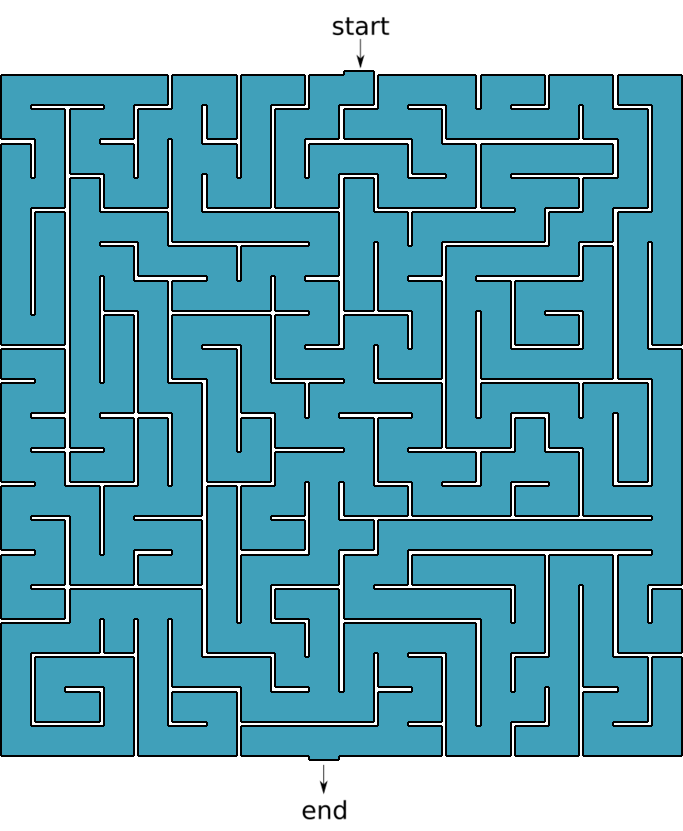
\includegraphics[width=\textwidth,height=8cm]{maze1.png}
\end{column}

\begin{column}{0.5\textwidth}

\includegraphics[width=0.48\textwidth,height=\textheight]{homer.png}

\includegraphics[width=0.48\textwidth,height=\textheight]{homer2.png}

\begin{enumerate}
\tightlist
\item
  Go to \url{http://www.mazegenerator.net/}
\item
  Create a maze
\item
  Download it in PNG
\item
  Perform some conversions

  \begin{itemize}
  \tightlist
  \item
    PNG \(\rightarrow\) PNM \(\rightarrow\) SVG \(\rightarrow\) DXF
    \(\rightarrow\) GEO
  \item
    Details in FeenoX Tutorial \#2
  \end{itemize}
\end{enumerate}
\end{column}
\end{columns}
\end{frame}

\begin{frame}[fragile]{How to solve a maze without AI 2/3}
\protect\hypertarget{how-to-solve-a-maze-without-ai-23}{}
\begin{columns}[T]
\begin{column}{0.5\textwidth}
\begin{enumerate}
\setcounter{enumi}{4}
\item
  Open it with Gmsh

  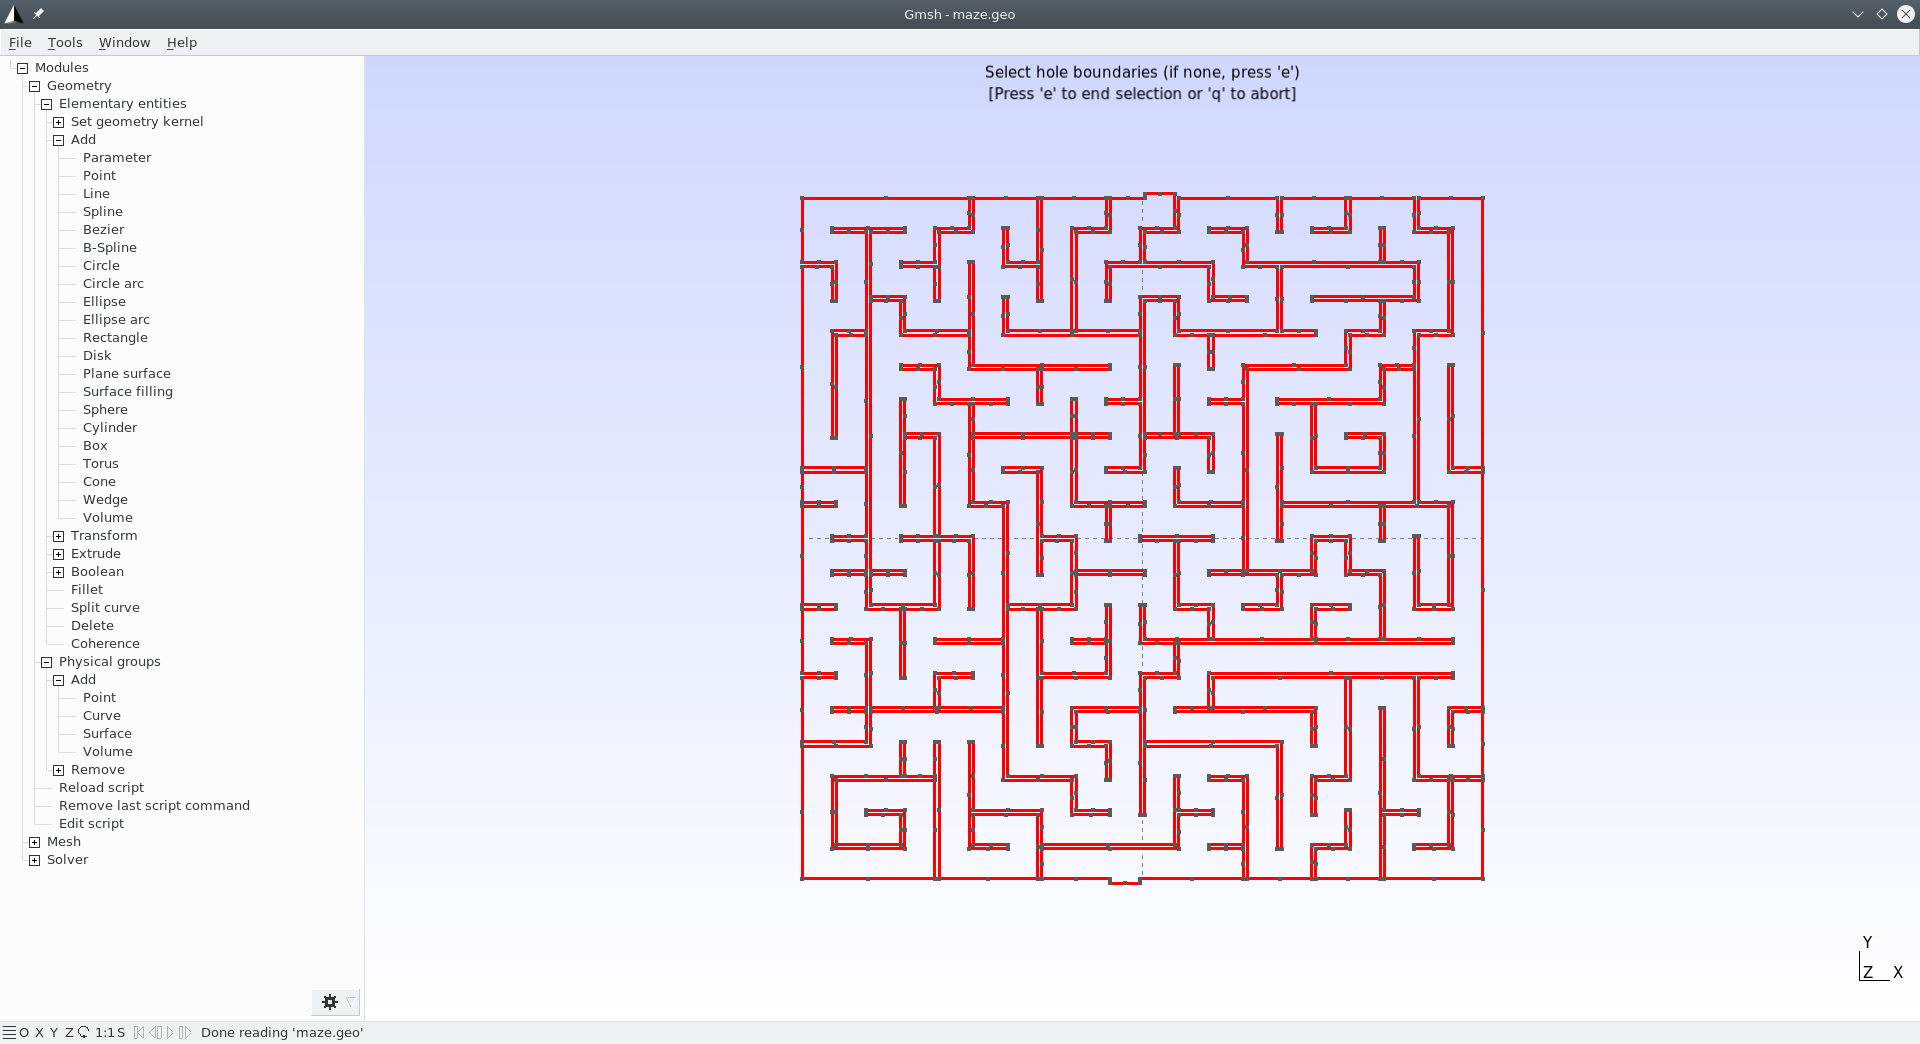
\includegraphics{gmsh-maze.png}~

  \begin{itemize}
  \tightlist
  \item
    Add a surface
  \item
    Set physical curves for ``start'' and ``end''
  \end{itemize}
\item
  Mesh it

\begin{lstlisting}[style=terminal]
gmsh -2 maze.geo
\end{lstlisting}
\end{enumerate}
\end{column}

\begin{column}{0.5\textwidth}
\centering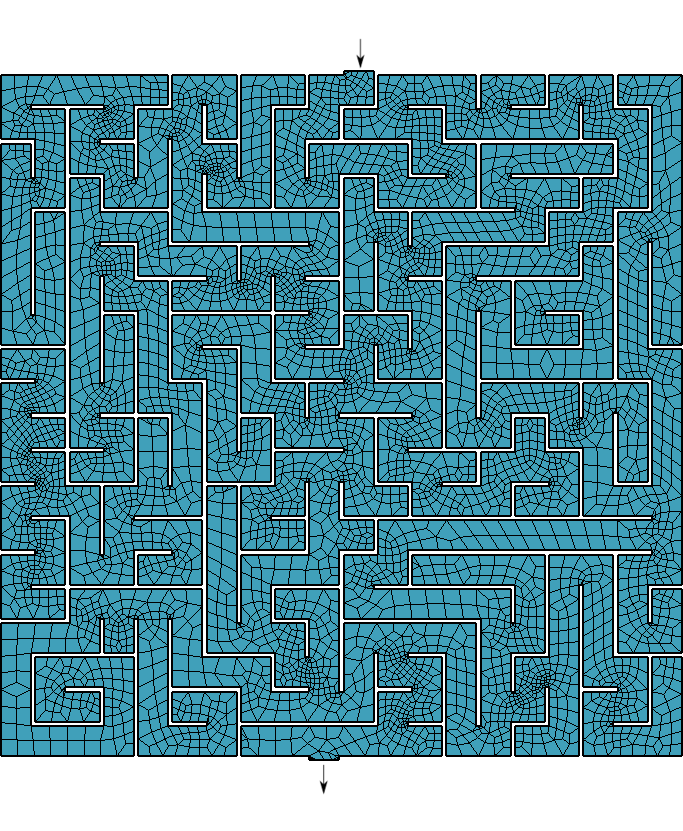
\includegraphics[height=8cm]{maze2.png}
\end{column}
\end{columns}
\end{frame}

\begin{frame}[fragile]{How to solve a maze without AI 3/3}
\protect\hypertarget{how-to-solve-a-maze-without-ai-33}{}
\begin{columns}[T]
\begin{column}{0.5\textwidth}
\begin{enumerate}
\setcounter{enumi}{6}
\item
  Solve \(\nabla^2 \phi = 0\) with BCs \vspace{-0.5cm} \[
  \begin{cases}
  \phi=0 & \text{at “start”} \\
  \phi=1 & \text{at “end”} \\
  \nabla \phi \cdot \hat{\mathbf{n}} = 0 & \text{everywhere else} \\
  \end{cases}
  \]

  \vspace{-0.5cm}

\begin{lstlisting}[style=feenox]
PROBLEM laplace 2D  # pretty self-descriptive, isn't it?
READ_MESH maze.msh

# boundary conditions (default is homogeneous Neumann)
BC start  phi=0 
BC end    phi=1

SOLVE_PROBLEM

# write the norm of gradient as a scalar field
# and the gradient as a 2d vector into a .msh file
WRITE_MESH maze-solved.msh \
    sqrt(dphidx(x,y)^2+dphidy(x,y)^2) \
    VECTOR dphidx dphidy 0 
\end{lstlisting}

\begin{lstlisting}[style=terminal]
$ feenox maze.fee
$
\end{lstlisting}

  \vspace{-0.25cm}\hfill{\footnotesize\textcolor{cyan}{(Rule of {silence})}}
\item
  Go to start and follow the gradient~\(\nabla \phi\)!
\end{enumerate}
\end{column}

\begin{column}{0.5\textwidth}
\only<1 | handout:0>{\centering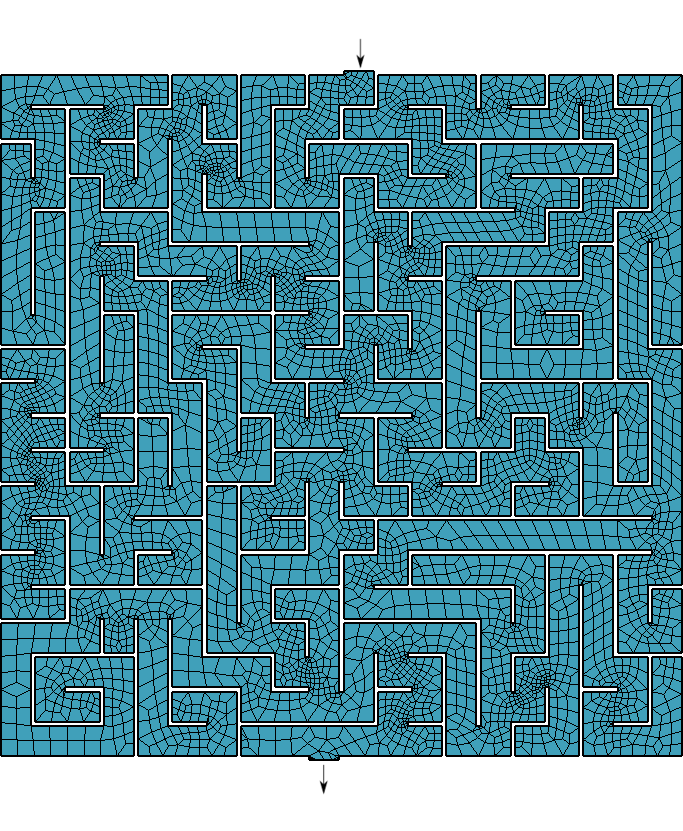
\includegraphics[height=8cm]{maze2.png}}\only<2>{\centering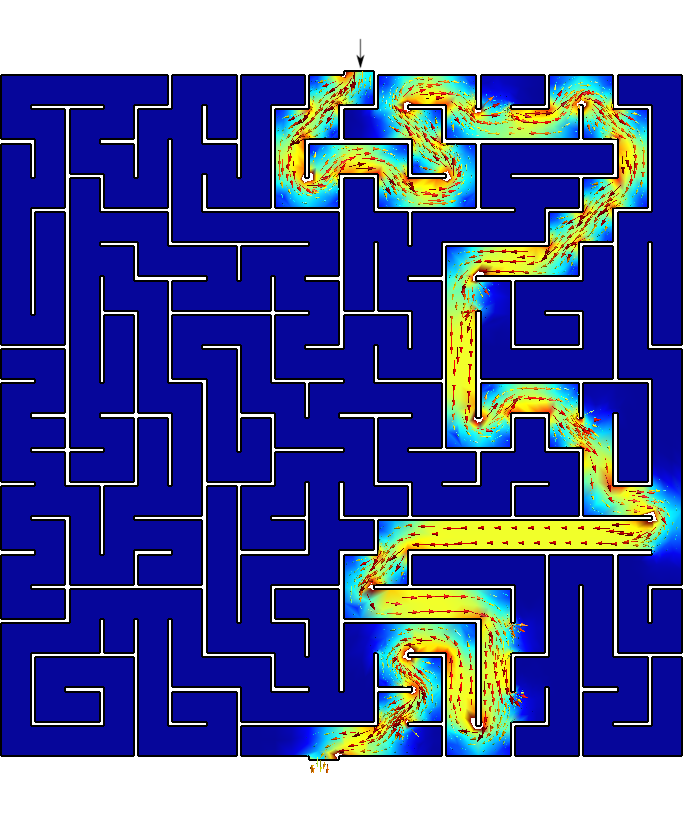
\includegraphics[height=8cm]{maze3.png}}
\end{column}
\end{columns}
\end{frame}

\begin{frame}{}
\protect\hypertarget{section-5}{}
\begin{columns}[T]
\begin{column}{0.5\textwidth}
\centering 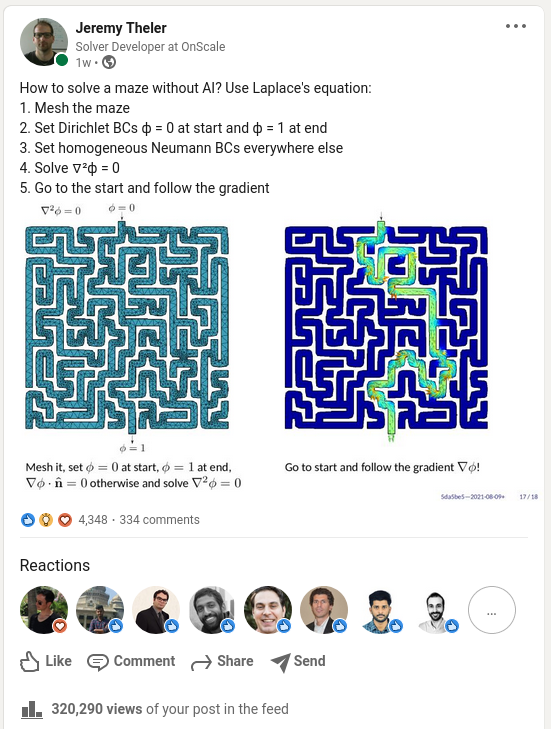
\includegraphics[width=0.8\textwidth,height=\textheight]{maze-linkedin3.png}
\end{column}

\begin{column}{0.5\textwidth}
\url{http://www.mazegenerator.net/Examples.aspx}

\centering 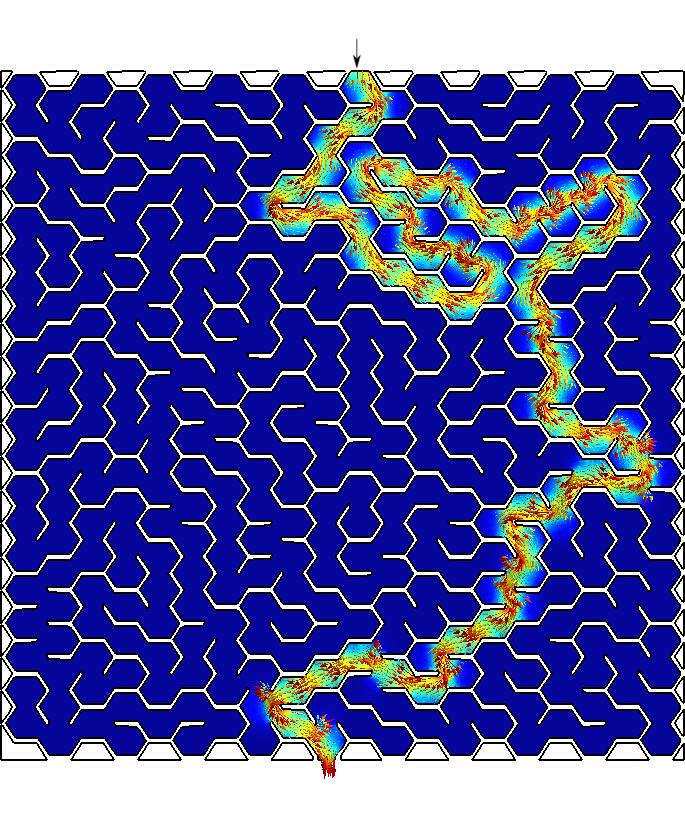
\includegraphics[width=0.45\textwidth,height=\textheight]{maze-sigma.png}
\centering 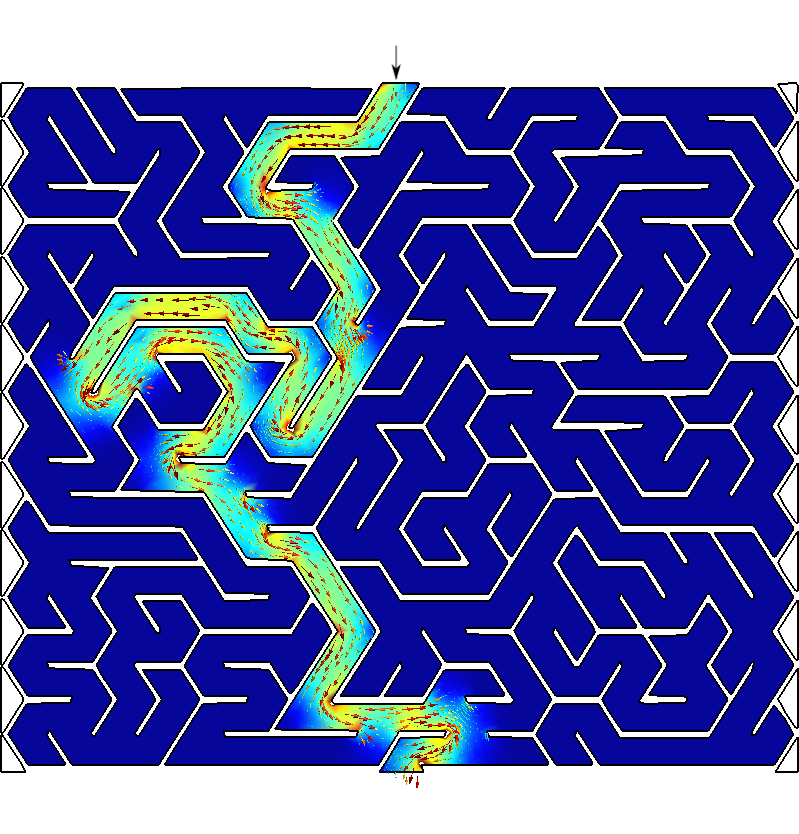
\includegraphics[width=0.45\textwidth,height=\textheight]{maze-delta.png}

\centering 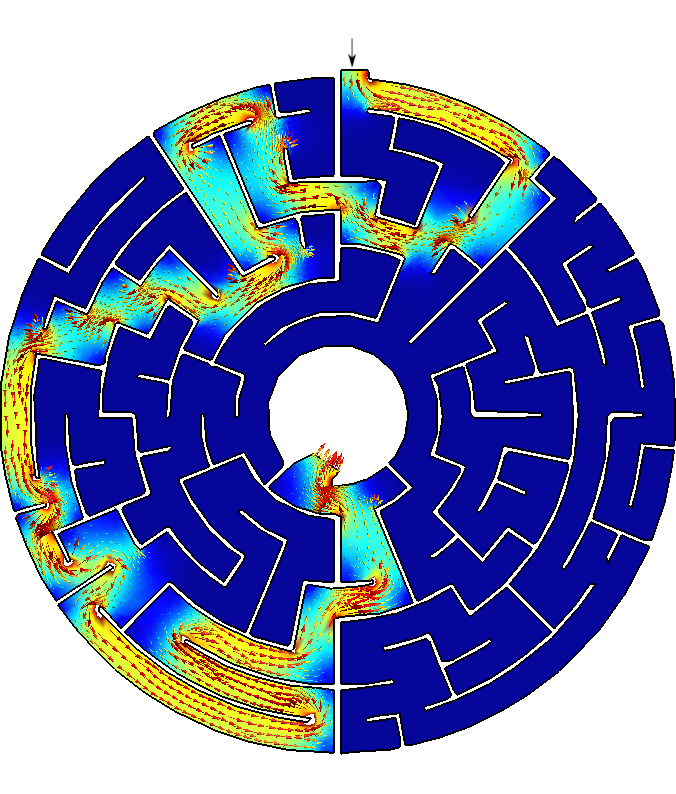
\includegraphics[width=0.45\textwidth,height=\textheight]{maze-theta.png}
\centering 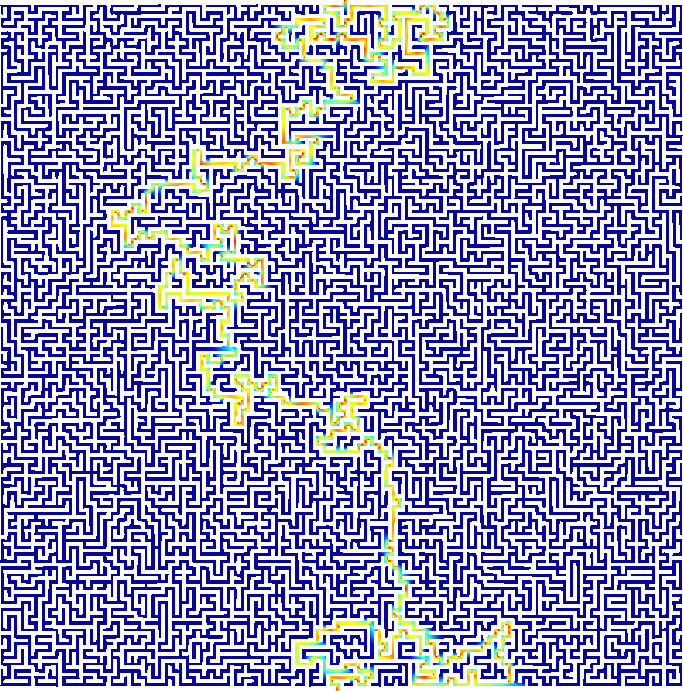
\includegraphics[width=0.45\textwidth,height=\textheight]{big-maze-solved.png}
\end{column}
\end{columns}
\end{frame}

\begin{frame}[fragile]{}
\protect\hypertarget{section-6}{}
\begin{columns}[T]
\begin{column}{0.5\textwidth}
\begin{block}{2.1. Deployment}
\protect\hypertarget{deployment}{}
\begin{itemize}
\tightlist
\item
  Automatically compile from source

  \begin{itemize}
  \tightlist
  \item
    Particular optimization flags
  \end{itemize}
\item
  Availability of pre-compiled binaries

  \begin{itemize}
  \tightlist
  \item
    Common architectures and options
  \end{itemize}
\item
  Both of them have to be available online
\end{itemize}
\end{block}

\begin{block}{2.2. Execution}
\protect\hypertarget{execution}{}
\begin{itemize}
\tightlist
\item
  Remote execution, either

  \begin{itemize}
  \tightlist
  \item
    By a direct user action
  \item
    From a higher-level workflow
  \end{itemize}
\item
  Outer loops have to be supported

  \begin{itemize}
  \tightlist
  \item
    scripted
  \item
    parametric
  \item
    optimization
  \end{itemize}
\item
  Ways to read data from the outer loop
\item
  Ways to write scalar figures of merit
\end{itemize}
\end{block}
\end{column}

\pause

\begin{column}{0.5\textwidth}
\begin{exampleblock}{FeenoX}
\protect\hypertarget{feenox-4}{}
\begin{itemize}
\item
  Compile optimized dependencies

\begin{lstlisting}[style=terminal]
$ cd $PETSC_DIR
$ export PETSC_ARCH=linux-fast
$ ./configure --with-debug=0 COPTFLAGS="-Ofast"
$ make -j8
\end{lstlisting}
\item
  Configure FeenoX with particular flags

\begin{lstlisting}[style=terminal]
$ git clone https://github.com/seamplex/feenox
$ cd feenox
$ ./autogen.sh
$ export PETSC_ARCH=linux-fast
$ ./configure MPICH_CC=clang CFLAGS=-Ofast
$ make -j8
# make install
\end{lstlisting}
\item
  Or use pre-compiled binaries

\begin{lstlisting}[style=terminal]
wget http://gmsh.info/bin/Linux/gmsh-Linux64.tgz
wget https://seamplex.com/feenox/dist/linux/feenox-linux-amd64.tar.gz
\end{lstlisting}
\item
  Everything is Docker-friendly
\item
  Execution examples follow \(\rightarrow\)
\end{itemize}
\end{exampleblock}
\end{column}
\end{columns}
\end{frame}

\begin{frame}[fragile]{Direct execution: three ways of getting the first
20 Fibonacci numbers}
\protect\hypertarget{direct-execution-three-ways-of-getting-the-first-20-fibonacci-numbers}{}
\begin{columns}[T]
\begin{column}{0.6\textwidth}
\begin{lstlisting}[style=feenox]
# the Fibonacci sequence using the closed-form formula as a function
phi = (1+sqrt(5))/2 
f(n) = (phi^n - (1-phi)^n)/sqrt(5)
PRINT_FUNCTION f MIN 1 MAX 20 STEP 1
\end{lstlisting}

\pause

\begin{lstlisting}[style=feenox]
# the fibonacci sequence as a vector
VECTOR f SIZE 20

f[i]<1:2> = 1
f[i]<3:vecsize(f)> = f[i-2] + f[i-1]

PRINT_VECTOR i f
\end{lstlisting}

\pause

\begin{lstlisting}[style=feenox]
# the fibonacci sequence as an iterative problem

static_steps = 20
#static_iterations = 1476  # limit of doubles

IF step_static=1|step_static=2
 f_n = 1
 f_nminus1 = 1
 f_nminus2 = 1
ELSE
 f_n = f_nminus1 + f_nminus2
 f_nminus2 = f_nminus1
 f_nminus1 = f_n
ENDIF

PRINT step_static f_n
\end{lstlisting}
\end{column}

\pause

\begin{column}{0.4\textwidth}
\begin{lstlisting}[style=terminal]
$ feenox fibo_formula.fee | tee one
1   1
2   1
3   2
4   3
5   5
6   8
7   13
8   21
9   34
10  55
11  89
12  144
13  233
14  377
15  610
16  987
17  1597
18  2584
19  4181
20  6765
$ feenox fibo_vector.fee > two
$ feenox fibo_iterative.fee > three
$ diff one two
$ diff two three
$
\end{lstlisting}
\end{column}
\end{columns}
\end{frame}

\begin{frame}[fragile]{Parametric execution: shear locking in
cantilevered beam}
\protect\hypertarget{parametric-execution-shear-locking-in-cantilevered-beam}{}
\begin{columns}[T]
\begin{column}{0.6\textwidth}
\begin{lstlisting}[language=bash, style=bash]
#!/bin/bash

rm -f *.dat
for element in tet4 tet10 hex8 hex20 hex27; do
 for c in $(seq 1 10); do
 
  # create mesh if not alreay cached
  mesh=cantilever-${element}-${c}
  if [ ! -e ${mesh}.msh ]; then
    scale=$(echo "PRINT 1/${c}" | feenox -)
    gmsh -3 -v 0 cantilever-${element}.geo -clscale ${scale} -o ${mesh}.msh
  fi
  
  # call FeenoX
  feenox cantilever.fee ${element} ${c} | tee -a cantilever-${element}.dat
  
 done
done
\end{lstlisting}

\begin{lstlisting}[style=feenox]
PROBLEM elastic 3D
READ_MESH cantilever-$1-$2.msh   # in meters

E = 2.1e11         # Young modulus in Pascals
nu = 0.3           # Poisson's ratio

BC left   fixed
BC right  tz=-1e5  # traction in Pascals, negative z
 
SOLVE_PROBLEM

# z-displacement (components are u,v,w) at the tip vs. number of nodes
PRINT nodes w(500,0,0) "\# $1 $2"
\end{lstlisting}

\vspace{-0.25cm}\hfill{\footnotesize\textcolor{cyan}{(Rule of {generation})}}
\end{column}

\begin{column}{0.4\textwidth}
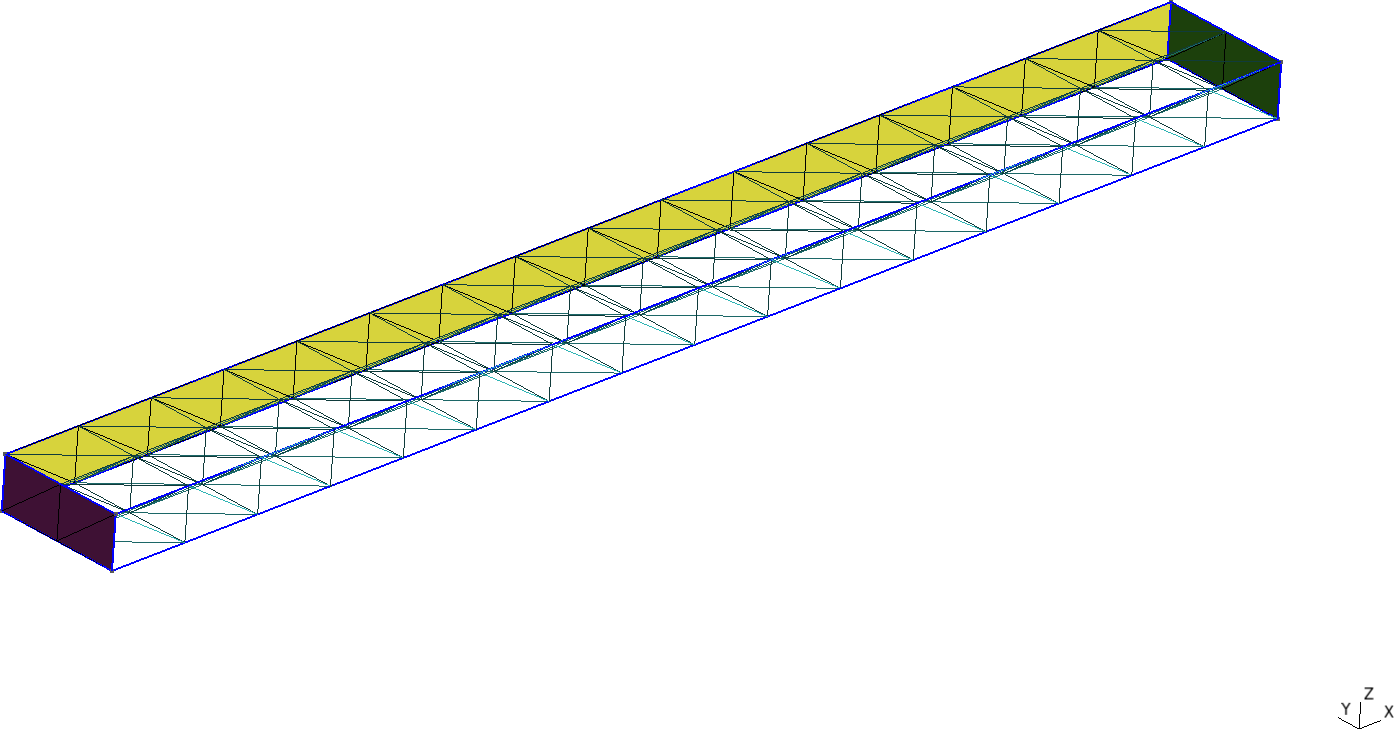
\includegraphics{cantilever-tet.png}

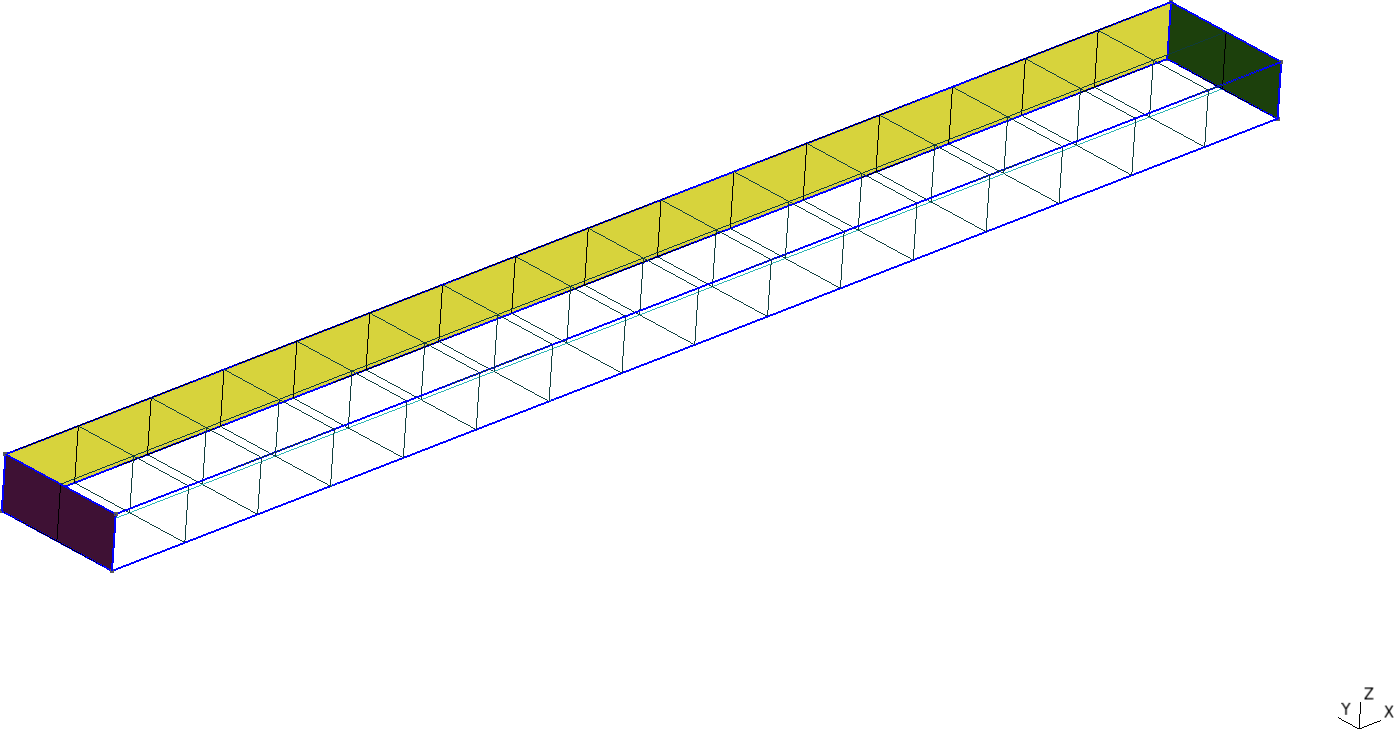
\includegraphics{cantilever-hex.png}

\begin{itemize}
\item
  {\textcolor{cyan}{Rule of {simplicity}}}

  \begin{itemize}
  \tightlist
  \item
    Only one material, no need to link volumes with materials
  \end{itemize}

\begin{lstlisting}[style=feenox]
E = 2.1e11   # Young modulus in Pa
\end{lstlisting}
\end{itemize}
\end{column}
\end{columns}
\end{frame}

\begin{frame}{Parametric execution: shear locking in cantilevered beam}
\protect\hypertarget{parametric-execution-shear-locking-in-cantilevered-beam-1}{}
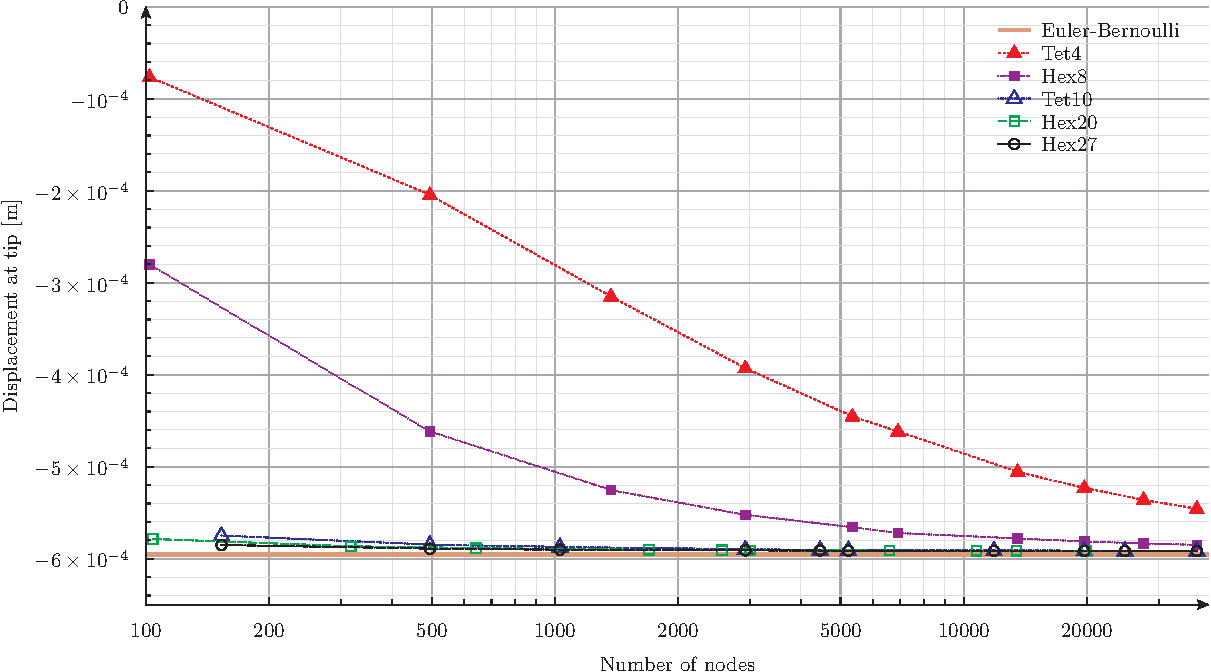
\includegraphics{cantilever-displacement.pdf}
\end{frame}

\begin{frame}[fragile]{Optimization loop: finding the right length of a
tuning fork}
\protect\hypertarget{optimization-loop-finding-the-right-length-of-a-tuning-fork}{}
\begin{columns}[T]
\begin{column}{0.2\textwidth}
\centering 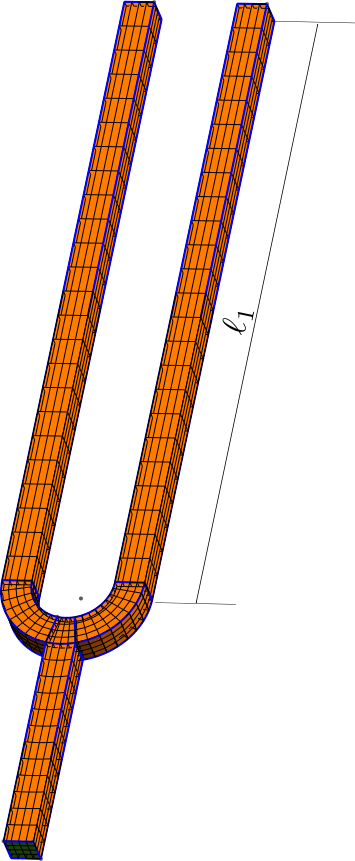
\includegraphics{fork-meshed.svg}

\(\ell_1\) to have 440~Hz?
\end{column}

\pause

\begin{column}{0.4\textwidth}
\begin{lstlisting}[language=Python, style=python]
import math
import gmsh
import subprocess  # to call FeenoX and read back

def create_mesh(r, w, l1, l2, n):
  gmsh.initialize()
  ...
  gmsh.finalize()
  return len(nodes)
  
def main():
  target = 440    # target frequency
  eps = 1e-2      # tolerance
  r = 4.2e-3      # geometric parameters
  w = 3e-3
  l1 = 30e-3
  l2 = 60e-3

  for n in range(1,7):   # mesh refinement level
    l1 = 60e-3              # restart l1 & error
    error = 60
    while abs(error) > eps:   # loop
      l1 = l1 - 1e-4*error
      # mesh with Gmsh Python API
      nodes = create_mesh(r, w, l1, l2, n)
      # call FeenoX and read scalar back
      # TODO: FeenoX Python API (like Gmsh)
      result = subprocess.run(['feenox', 'fork.fee'], stdout=subprocess.PIPE)
      freq = float(result.stdout.decode('utf-8'))
      error = target - freq
    
    print(nodes, l1, freq)
\end{lstlisting}

\vspace{-0.25cm}\hfill{\footnotesize\textcolor{cyan}{(Rule of {parsimony})}}
\end{column}

\begin{column}{0.4\textwidth}
\begin{lstlisting}[style=feenox]
PROBLEM modal 3D MODES 1  # only one mode needed
READ_MESH fork.msh  # in [m]
E = 2.07e11         # in [Pa]
nu = 0.33
rho = 7829          # in [kg/m^2]

# no BCs! It is a free-free vibration problem
SOLVE_PROBLEM

# write back the fundamental frequency to stdout
PRINT f(1)
\end{lstlisting}

\vspace{-0.25cm}\hfill{\footnotesize\textcolor{cyan}{(Rule of {simplicity})}}

\pause

\begin{lstlisting}[style=terminal]
$ python fork.py > fork.dat
$
\end{lstlisting}

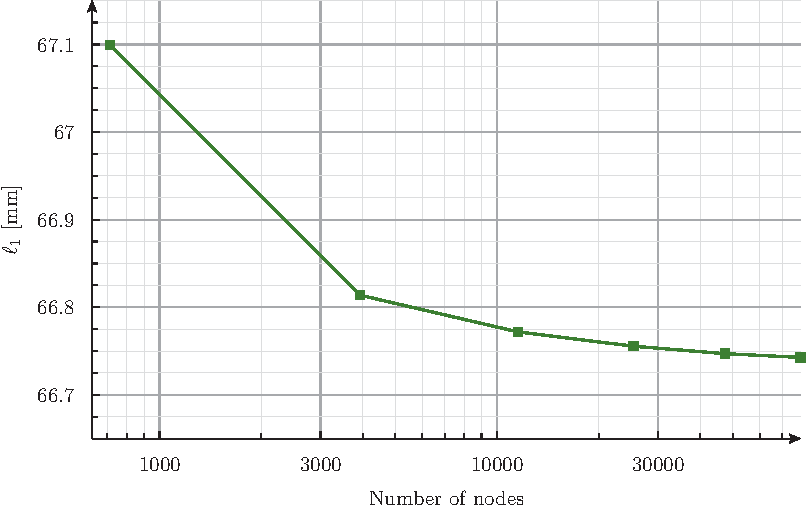
\includegraphics{fork.pdf}
\end{column}
\end{columns}
\end{frame}

\begin{frame}[fragile]{}
\protect\hypertarget{section-7}{}
\begin{columns}[T]
\begin{column}{0.475\textwidth}
\begin{block}{2.3. Efficiency}
\protect\hypertarget{efficiency}{}
\begin{itemize}
\tightlist
\item
  Similar to to other tools in terms of

  \begin{itemize}
  \tightlist
  \item
    CPU/GPU
  \item
    RAM
  \item
    Storage
  \end{itemize}
\end{itemize}
\end{block}

\begin{block}{2.4. Scalability}
\protect\hypertarget{scalability}{}
\begin{itemize}
\tightlist
\item
  Small problems to check correctness
\item
  Large problems in parallel

  \begin{itemize}
  \tightlist
  \item
    Reasonable weak \& strong scalability
  \end{itemize}
\end{itemize}
\end{block}

\begin{block}{2.5. Flexibility}
\protect\hypertarget{flexibility}{}
\begin{itemize}
\tightlist
\item
  Engineering problems with

  \begin{itemize}
  \tightlist
  \item
    Multiple materials
  \item
    Space-dependent properties
  \item
    Space \& time-dependent BCs
  \end{itemize}
\item
  Handle point-wise data

  \begin{itemize}
  \tightlist
  \item
    Properties
  \item
    Time-dependent scalars
  \end{itemize}
\end{itemize}
\end{block}
\end{column}

\pause

\begin{column}{0.525\textwidth}
\begin{exampleblock}{FeenoX}
\protect\hypertarget{feenox-5}{}
\begin{itemize}
\tightlist
\item
  First make it work, then optimize

  \begin{itemize}
  \item
    {\textcolor{cyan}{Rule of {optimization}}}
  \item
    https://seamplex.com/feenox/tests/nafems/le10/
  \end{itemize}
\item
  Linear solvers

  \begin{itemize}
  \tightlist
  \item
    Direct solver MUMPS

    \begin{itemize}
    \tightlist
    \item
      Robust but not scalable
    \end{itemize}
  \item
    GAMG-preconditioned KSP

    \begin{itemize}
    \tightlist
    \item
      Near-nullspace improves convergence
    \end{itemize}
  \end{itemize}
\item
  Non-linear \& transient solvers

  \begin{itemize}
  \tightlist
  \item
    Scalable as PETSc
  \end{itemize}
\item
  Written in ANSI C99 (no C++ nor Fortran)

  \begin{itemize}
  \item
    Autotools \& friends, POSIX
  \item
    Tested with \passthrough{\lstinline!gcc!},
    \passthrough{\lstinline!clang!} and \passthrough{\lstinline!icc!}
  \item
    Rust \& Go, can't tell (yet)
  \item
    {\textcolor{cyan}{Rule of {transparency}}}
  \end{itemize}
\item
  Flexibility follows \(\rightarrow\)
\end{itemize}
\end{exampleblock}
\end{column}
\end{columns}
\end{frame}

\begin{frame}[fragile]{Flexibility I: one-dimensional thermal slab}
\protect\hypertarget{flexibility-i-one-dimensional-thermal-slab}{}
\begin{columns}[T]
\begin{column}{0.45\textwidth}
Solve heat conduction on the slab \(x \in [0:1]\) with boundary
conditions

\[
\begin{cases}
T(0) = 0 & \text{(left)} \\
T(1) = 1 & \text{(right)} \\
\end{cases}
\]

\noindent and uniform conductivity. Compute
\(T\left(\frac{1}{2}\right)\).

\pause

\begin{itemize}
\tightlist
\item
  English self-evident ASCII input

  \begin{itemize}
  \tightlist
  \item
    Syntactic sugar
  \item
    Simple problems, simple inputs
  \end{itemize}
\item
  Mesh separated from problem

  \begin{itemize}
  \tightlist
  \item
    Git-friendly \passthrough{\lstinline!.geo!} \&
    \passthrough{\lstinline!.fee!}
  \end{itemize}
\item
  Output is 100\% user-defined

  \begin{itemize}
  \item
    No \passthrough{\lstinline!PRINT!} no output
  \item
    {\textcolor{cyan}{Rule of {silence}}}
  \end{itemize}
\item
  There is no node at \(x=1/2=0.5\)!
\end{itemize}
\end{column}

\begin{column}{0.55\textwidth}
\begin{lstlisting}[language=C, style=c]
Point(1) = {0, 0, 0};          // geometry: 
Point(2) = {1, 0, 0};          // two points
Line(1) = {1, 2};              // and a line connecting them!

Physical Point("left") = {1};  // groups for BCs and materials
Physical Point("right") = {2};
Physical Line("bulk") = {1};   // needed due to how Gmsh works

Mesh.MeshSizeMax = 1/3;        // mesh size, three line elements
Mesh.MeshSizeMin = Mesh.MeshSizeMax;
\end{lstlisting}

\vspace{-0.25cm}\hfill{\footnotesize\textcolor{cyan}{(Rule of {composition})}}

\begin{lstlisting}[style=feenox]
PROBLEM thermal 1D    # tell FeenoX what we want to solve 
READ_MESH slab.msh    # read mesh in Gmsh's v4.1 format
k = 1                 # set uniform conductivity
BC left  T=0          # set fixed temperatures as BCs
BC right T=1          # "left" and "right" are defined in the mesh
SOLVE_PROBLEM         # we are ready to solve the problem
PRINT T(1/2)          # ask for the temperature at x=1/2
\end{lstlisting}

\vspace{-0.25cm}\hfill{\footnotesize\textcolor{cyan}{(Rule of {simplicity})}}

\begin{lstlisting}[style=terminal]
$ gmsh -1 slab.geo
[...]
Info    : 4 nodes 5 elements
Info    : Writing 'slab.msh'...
[...]
$ feenox thermal-1d-dirichlet-uniform-k.fee 
0.5
$ 
\end{lstlisting}

\vspace{-0.25cm}\hfill{\footnotesize\textcolor{cyan}{(Rule of {economy})}}
\end{column}
\end{columns}
\end{frame}

\begin{frame}[fragile]{Flexibility II: one-dimensional thermal slabs}
\protect\hypertarget{flexibility-ii-one-dimensional-thermal-slabs}{}
\begin{columns}[T]
\begin{column}{0.45\textwidth}
\begin{lstlisting}[style=feenox]
PROBLEM heat 1D
READ_MESH slab.msh

BC left  T=0
BC right T=1

INCLUDE $1.fee   # read k and solution from $1

SOLVE_PROBLEM

PRINT_FUNCTION T T_analytical MIN 0 MAX 1 NSTEPS 100
\end{lstlisting}

\begin{lstlisting}[style=feenox]
k = 1            # uniform.fee
T_analytical(x) = x
\end{lstlisting}

\begin{lstlisting}[style=feenox]
k(x) = 1+x       # space.fee
T_analytical(x) = log(1+x)/log(2)
\end{lstlisting}

\begin{lstlisting}[style=feenox]
a = 2            # temperature.fee
k(x) = 1+a*T(x)
T_analytical(x) = (1/a)*(sqrt(1+(2+a)*a*x)-1)
\end{lstlisting}

\pause

\begin{itemize}
\tightlist
\item
  Everything is an expression
\item
  Similar problems need similar inputs
\item
  {\textcolor{cyan}{Rule of {least surprise}}}: \(k(x)=1+x\)
\end{itemize}
\end{column}

\begin{column}{0.55\textwidth}
\begin{lstlisting}[language=bash, style=bash]
for i in uniform space temperature; do
  feenox thermal-1d-dirichlet.fee ${i} > ${i}.dat
done
\end{lstlisting}

\centering 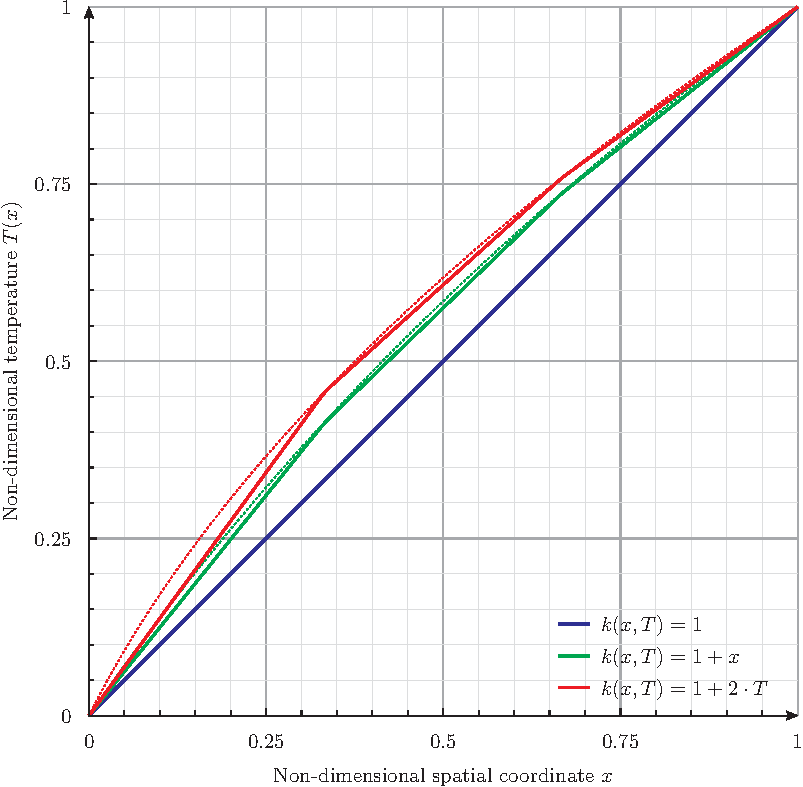
\includegraphics[width=0.75\textwidth,height=\textheight]{thermal-slabs.pdf}

\begin{itemize}
\tightlist
\item
  FeenoX can tell that \(k(T)\) is non-linear

  \begin{itemize}
  \tightlist
  \item
    It switchs from
    \href{https://petsc.org/release/docs/manual/ksp/}{\passthrough{\lstinline!KSP!}}
    to
    \href{https://petsc.org/release/docs/manual/snes/}{\passthrough{\lstinline!SNES!}}
  \end{itemize}
\end{itemize}
\end{column}
\end{columns}
\end{frame}

\begin{frame}[fragile]{Flexibility III: two squares in thermal contact}
\protect\hypertarget{flexibility-iii-two-squares-in-thermal-contact}{}
\begin{columns}[T]
\begin{column}{0.5\textwidth}
\centering 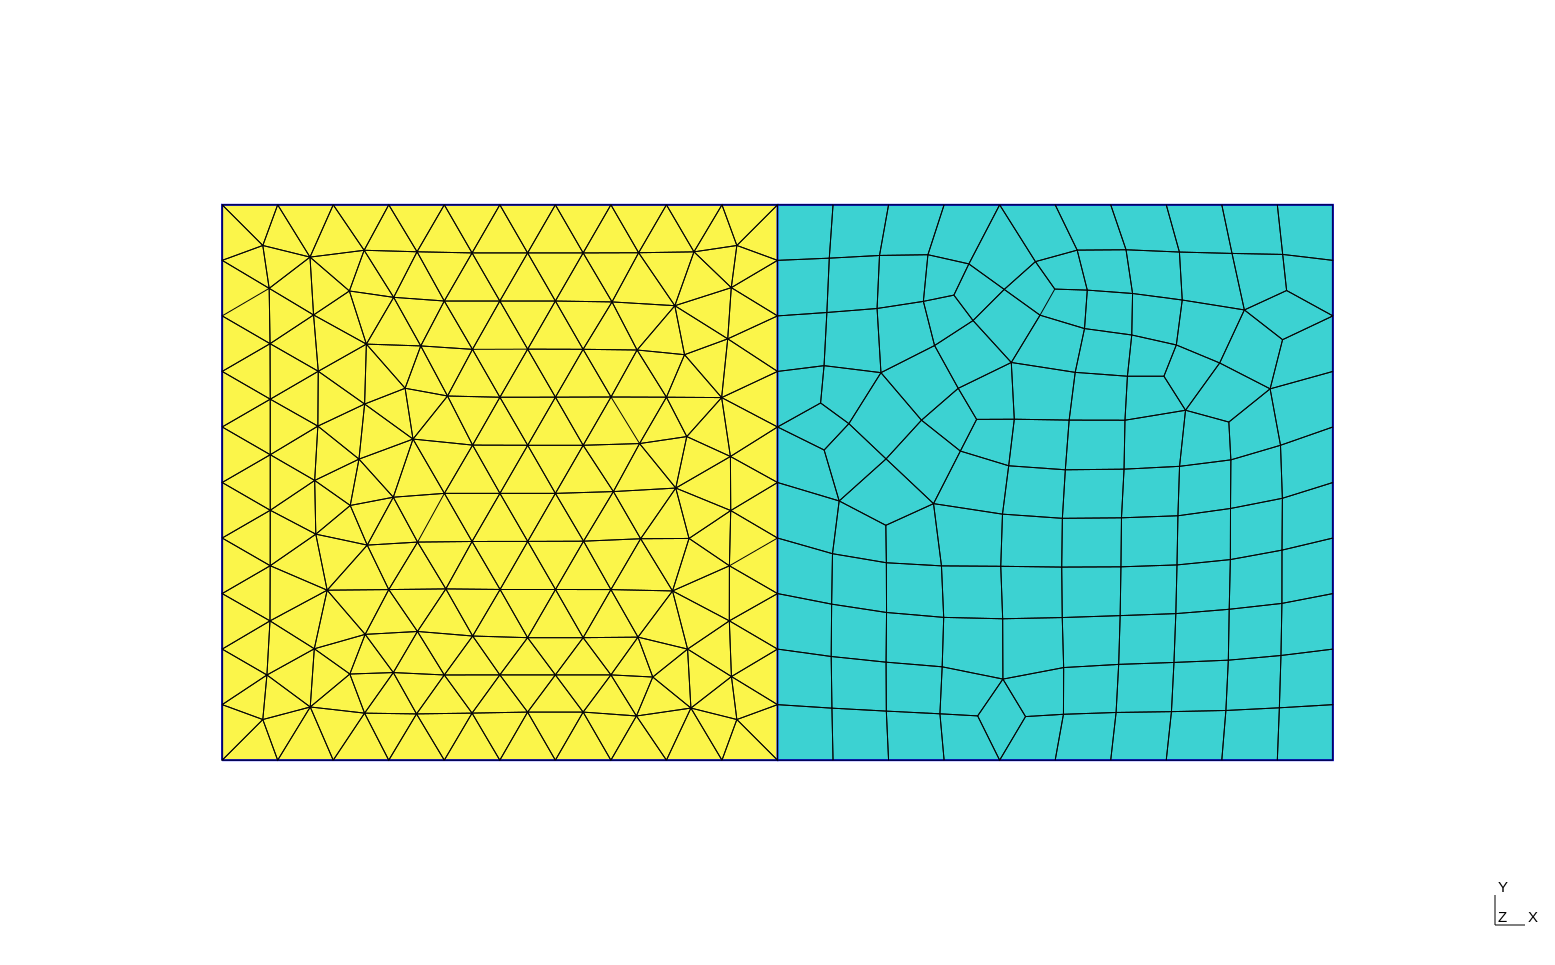
\includegraphics[width=0.65\textwidth,height=\textheight]{two-squares-mesh.svg}

\begin{lstlisting}[style=feenox]
PROBLEM thermal 2d
READ_MESH two-squares.msh

FUNCTION cond(x,y) INTERPOLATION shepard DATA {
    1   0    1.0
    1   1    1.5
    2   0    1.3
    2   1    1.8
    1.5 0.5  1.7 }

#        name   conductivity  power density
MATERIAL yellow k=0.5+T(x,y)  q=0
MATERIAL cyan   k=cond(x,y)   q=1-0.2*T(x,y)
    
BC left   T=y              # temperature
BC bottom T=1-cos(pi/2*x)
BC right  q=2-y            # heat flux
BC top    q=1

SOLVE_PROBLEM
 
WRITE_MESH two-squares.vtk  T CELLS k
\end{lstlisting}

\vspace{-0.25cm}\hfill{\footnotesize\textcolor{cyan}{(Rule of {clarity})}}
\end{column}

\pause

\begin{column}{0.5\textwidth}
\centering 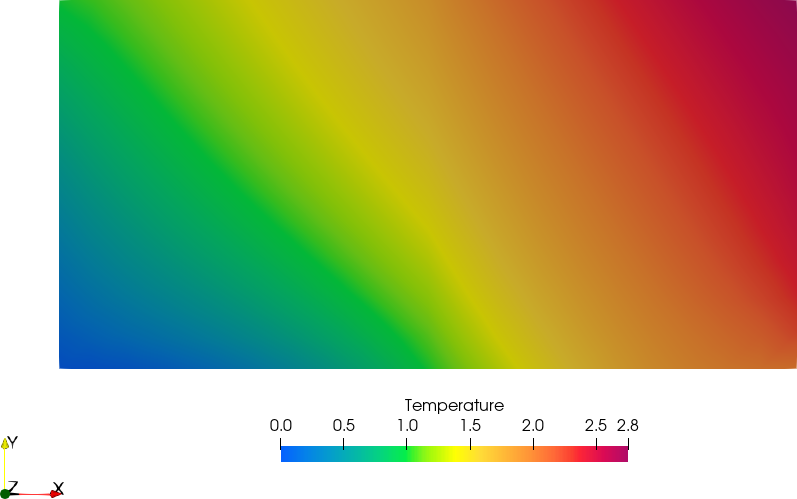
\includegraphics[width=0.7\textwidth,height=\textheight]{two-squares-temperature.png}

\centering 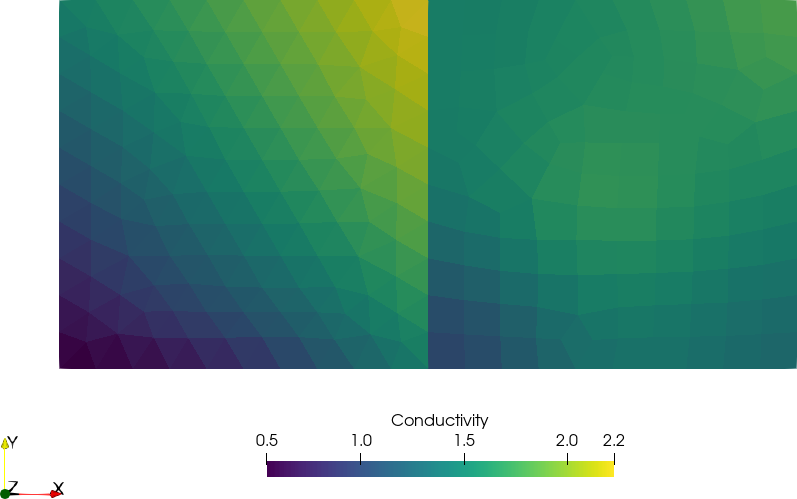
\includegraphics[width=0.7\textwidth,height=\textheight]{two-squares-conductivity.png}

\begin{itemize}
\tightlist
\item
  Volumes \(\Leftrightarrow\) materials now needed
\item
  FeenoX detects the problem is non-linear
\item
  \textcolor{Orange}{TO-DO}: roughish output
\end{itemize}
\end{column}
\end{columns}
\end{frame}

\begin{frame}[fragile]{Flexibility IV: thermal transient with
time-dependent BCs}
\protect\hypertarget{flexibility-iv-thermal-transient-with-time-dependent-bcs}{}
\begin{columns}[T]
\begin{column}{0.5\textwidth}
\centering 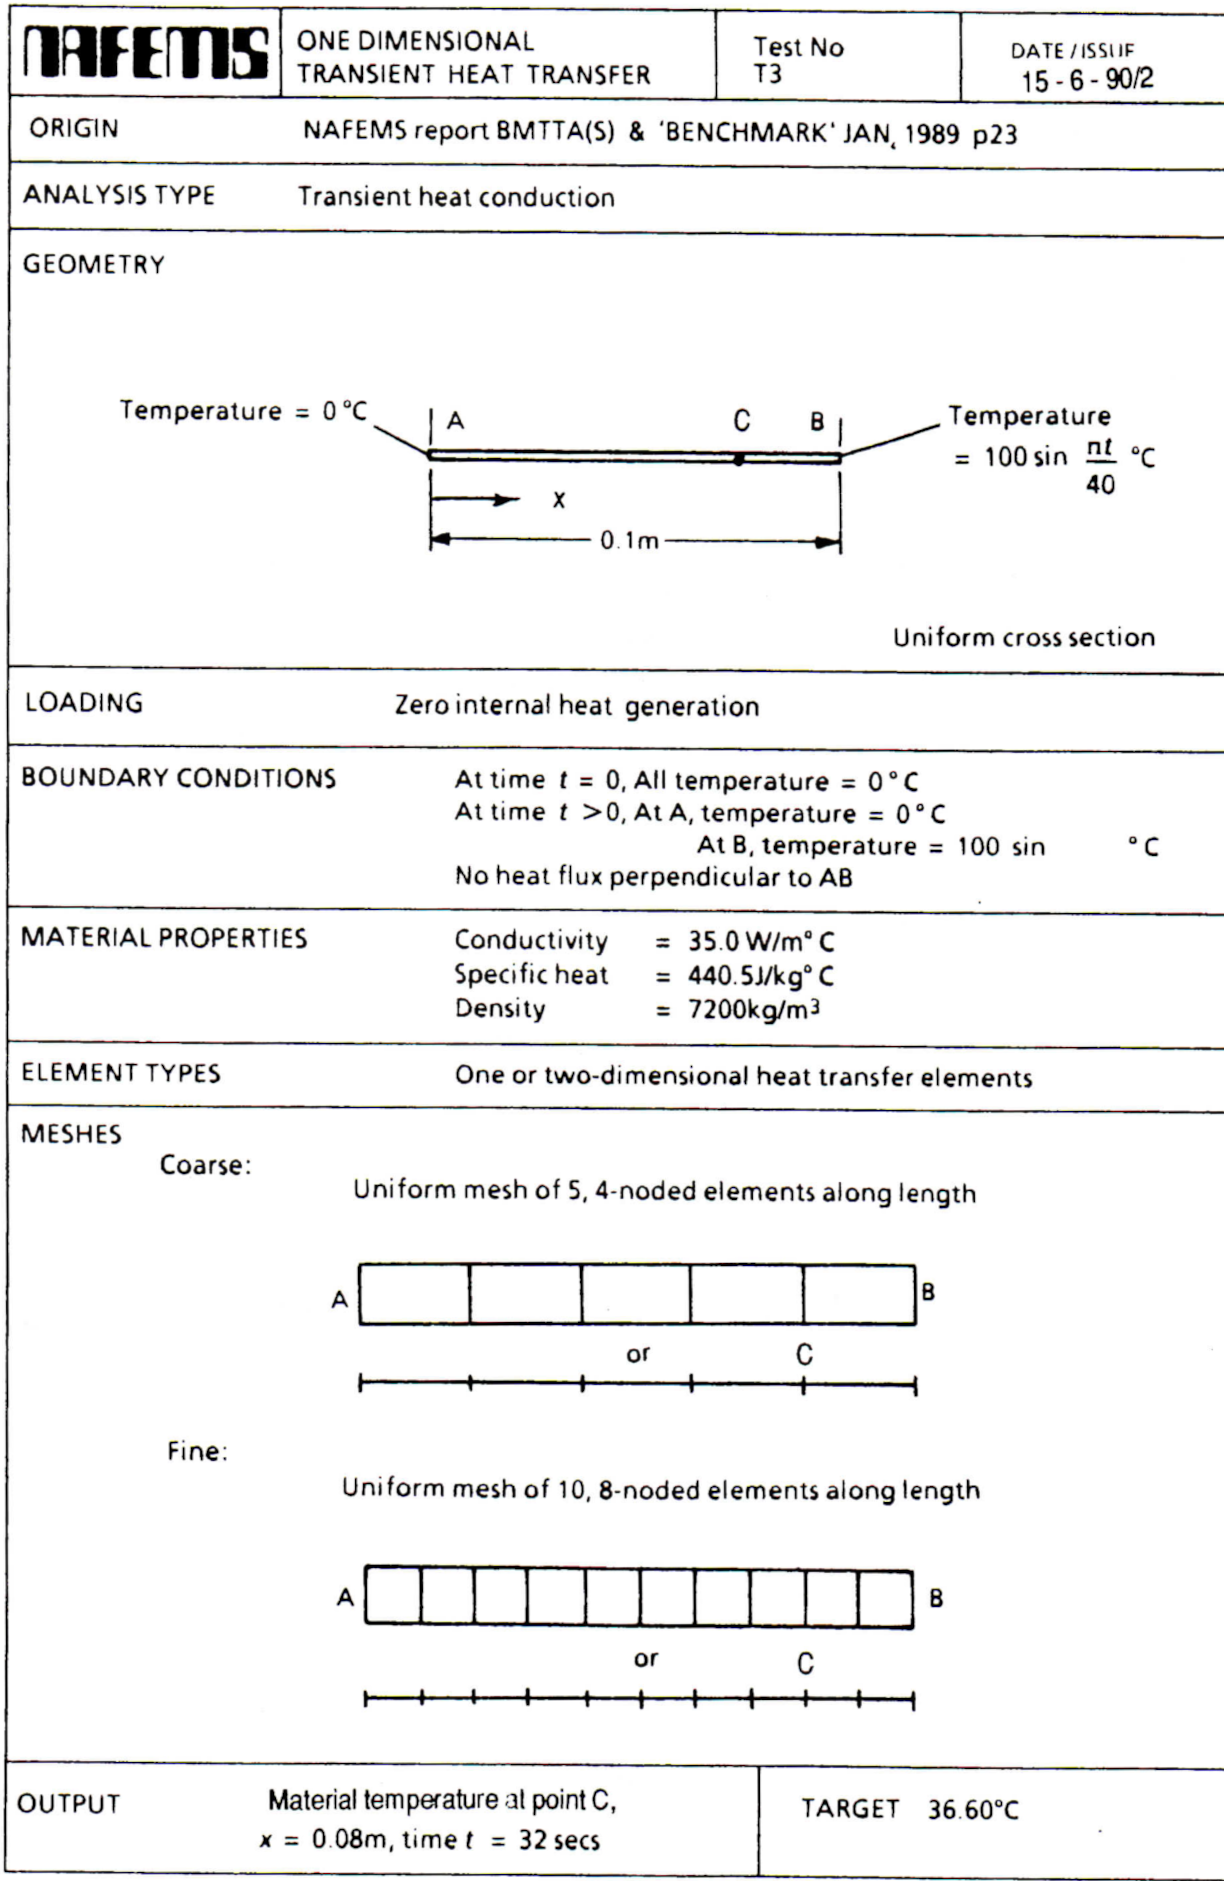
\includegraphics[width=0.75\textwidth,height=\textheight]{nafems-t3.png}
\end{column}

\pause

\begin{column}{0.5\textwidth}
\begin{lstlisting}[style=feenox]
# NAFEMS-T3 benchmark: 1d transient heat conduction
PROBLEM heat DIMENSIONS 1
READ_MESH slab-0.1m.msh

T_0(x) = 0         # initial condition

BC left  T=0       # prescribed temperatures
BC right T=100*sin(pi*t/40)

k = 35.0           # conductivity [W/(m K)]
cp = 440.5         # heat capacity [J/(kg K)]
rho = 7200         # density [kg/m^3]

end_time = 32      # trasient up to 32 seconds

SOLVE_PROBLEM

PRINT %.3f t dt %.2f T(0.1) T(0.08) 

IF done
 PRINT "\# result = " T(0.08) "ºC"
ENDIF
\end{lstlisting}

\begin{lstlisting}[style=terminal]
$ feenox nafems-t3.fee 
0.000   0.062   0.00    0.00
0.002   0.002   0.01    0.00
[...]
30.871  0.565   65.71   36.04
31.435  0.565   62.31   36.33
32.000  1.050   58.78   36.56
# result =      36.5636 ºC
$
\end{lstlisting}
\end{column}
\end{columns}
\end{frame}

\begin{frame}{}
\protect\hypertarget{section-8}{}
\begin{columns}[T]
\begin{column}{0.5\textwidth}
\begin{block}{2.6. Extensibility}
\protect\hypertarget{extensibility}{}
\begin{itemize}
\tightlist
\item
  Possibility to add more features

  \begin{itemize}
  \tightlist
  \item
    More PDEs
  \item
    New material models (i.e.~stress-strain)
  \item
    Other element types
  \end{itemize}
\item
  Clear licensing scheme for extensions
\end{itemize}
\end{block}

\begin{block}{2.7. Interoperability}
\protect\hypertarget{interoperability}{}
\begin{itemize}
\tightlist
\item
  Ability to exchange data with other tools following this SRS

  \begin{itemize}
  \tightlist
  \item
    Pre and post processors
  \item
    Optimization tools
  \item
    Coupled multi-physics calculations
  \end{itemize}
\end{itemize}
\end{block}
\end{column}

\pause

\begin{column}{0.5\textwidth}
\begin{exampleblock}{FeenoX}
\protect\hypertarget{feenox-6}{}
\begin{itemize}
\tightlist
\item
  Think for the future! {\textcolor{cyan}{Rule of {extensibility}}}

  \begin{itemize}
  \tightlist
  \item
    GPLv3\textbf{+}: the `+' is for the future
  \end{itemize}
\item
  Nice-to-haves: \textcolor{Orange}{TO-DO}

  \begin{itemize}
  \tightlist
  \item
    Lagrangian elements, DG, \(h\)-\(p\) AMR, \ldots{}
  \end{itemize}
\item
  Other problems \& formulations:

  \begin{itemize}
  \tightlist
  \item
    Each PDE has an independent directory
  \item
    ``Virtual methods'' as function pointers
  \item
    Use Laplace as a template (elliptic)
  \item
    Add or remove source directory
  \end{itemize}
\item
  Coupled calculations: \textcolor{Orange}{TO-DO}

  \begin{itemize}
  \tightlist
  \item
    Plain (RAM-disk) files
  \item
    Shared memory \& semaphores
  \item
    MPI
  \end{itemize}
\item
  Interoperability

  \begin{itemize}
  \tightlist
  \item
    Gnuplot, matplotlib, etc.
  \item
    Gmsh (+ Meshio), Paraview
  \item
    CAEplex
  \item
    PrePoMax, FreeCAD, \ldots: \textcolor{Orange}{TO-DO}
  \end{itemize}
\end{itemize}
\end{exampleblock}
\end{column}
\end{columns}
\end{frame}

\begin{frame}[fragile]{Laplace equation with both Gmsh \& Paraview as
post-processors}
\protect\hypertarget{laplace-equation-with-both-gmsh-paraview-as-post-processors}{}
\begin{columns}[T]
\begin{column}{0.6\textwidth}
Solve \(\nabla^2 \phi = 0\) over \([-1:+1]\times[-1:+1]\) with

\[
\begin{cases}
\phi(x,y) = +y & \text{for $x=-1$ (left)} \\
\phi(x,y) = -y & \text{for $x=+1$ (right)} \\
\nabla \phi \cdot \hat{\mathbf{n}} = \sin\left(\frac{\pi}{2} x\right) & \text{for $y=-1$ (bottom)} \\
\nabla \phi \cdot \hat{\mathbf{n}} =0 & \text{for $y=+1$ (top)} \\
\end{cases}
\]

\begin{lstlisting}[style=feenox]
PROBLEM laplace 2d
READ_MESH square-centered.msh # [-1:+1]x[-1:+1]

# boundary conditions
BC left    phi=+y
BC right   phi=-y
BC bottom  dphidn=sin(pi/2*x)
BC top     dphidn=0

SOLVE_PROBLEM

# same output in .msh and in .vtk formats
WRITE_MESH laplace-square.msh phi VECTOR dphidx dphidy 0
WRITE_MESH laplace-square.vtk phi VECTOR dphidx dphidy 0
\end{lstlisting}

\vspace{-0.25cm}\hfill{\footnotesize\textcolor{cyan}{(Rule of {diversity})}}
\end{column}

\pause

\begin{column}{0.4\textwidth}
\centering \hspace{0.5cm}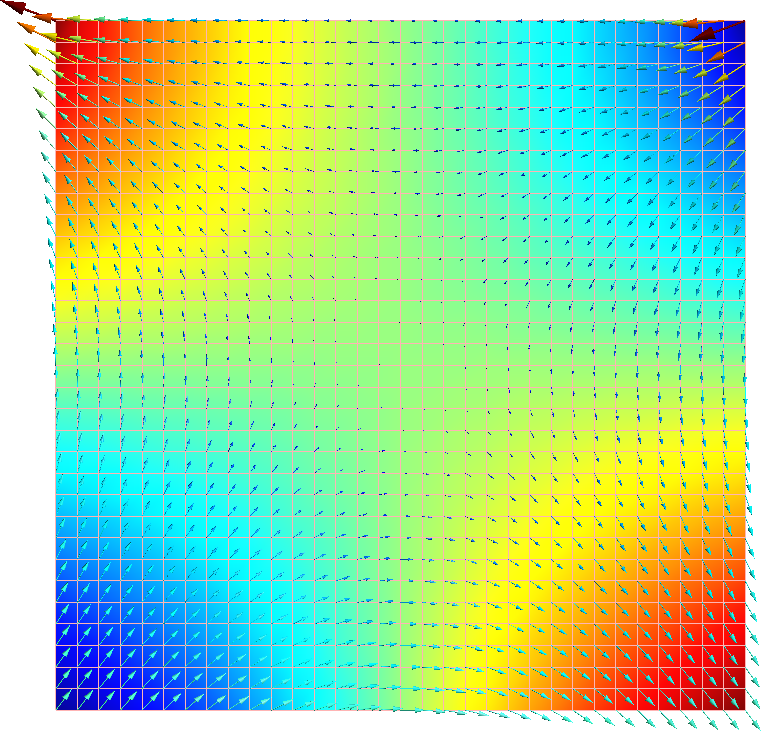
\includegraphics[width=0.7\textwidth,height=\textheight]{laplace-square-gmsh.png}\\

\centering 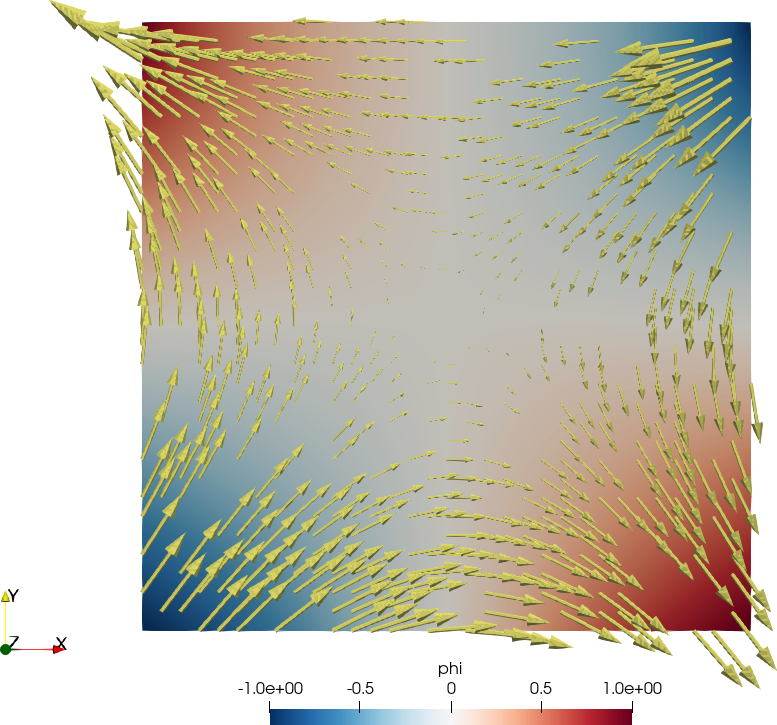
\includegraphics[width=0.8\textwidth,height=\textheight]{laplace-square-paraview.png}\\
\end{column}
\end{columns}
\end{frame}

\begin{frame}[fragile]{}
\protect\hypertarget{section-9}{}
\begin{columns}[T]
\begin{column}{0.5\textwidth}
\begin{block}{3. Interfaces}
\protect\hypertarget{interfaces}{}
\begin{itemize}
\tightlist
\item
  Fully human-less execution

  \begin{itemize}
  \tightlist
  \item
    Input files (1 or more)
  \item
    Output files (0 or more)
  \end{itemize}
\item
  Ability to remotely report status

  \begin{itemize}
  \tightlist
  \item
    Progress
  \item
    Errors
  \end{itemize}
\end{itemize}

\begin{block}{3.1. Input}
\protect\hypertarget{input}{}
\begin{itemize}
\tightlist
\item
  Problem fully defined in input files

  \begin{itemize}
  \tightlist
  \item
    Ad-hoc syntax
  \item
    API for high-level languages
  \item
    Other files (data, meshes, scripts)
  \end{itemize}
\item
  Preferably ASCII (for DCVS)

  \begin{itemize}
  \tightlist
  \item
    Avoid mixing problem and mesh data
  \end{itemize}
\item
  GUI not mandatory but possible

  \begin{itemize}
  \tightlist
  \item
    Ok to have basic usage through GUI
  \item
    Advanced features through API
  \end{itemize}
\end{itemize}
\end{block}
\end{block}
\end{column}

\pause

\begin{column}{0.5\textwidth}
\begin{exampleblock}{FeenoX}
\protect\hypertarget{feenox-7}{}
\begin{itemize}
\tightlist
\item
  Human-less production workflow
\item
  There are ASCII progress bars

  \begin{itemize}
  \tightlist
  \item
    Build matrix
  \item
    Solve equations
  \item
    Gradient recovery
  \end{itemize}
\item
  Heartbeat: \textcolor{Orange}{TO-DO}
\end{itemize}

\medskip

\begin{itemize}
\tightlist
\item
  English self-evident ASCII input

  \begin{itemize}
  \item
    Syntactically-sugared

    \begin{itemize}
    \tightlist
    \item
      Nouns are definitions
    \item
      Verbs are instructions
    \end{itemize}
  \item
    Simple problems, simple inputs
  \item
    Similar problems, similar inputs
  \item
    Everything is an expression!
  \item
    {\textcolor{cyan}{Rule of {least surprise}}}:
    \(f(x)=\frac{1}{2} \cdot x^2\)

\begin{lstlisting}[style=feenox]
f(x) = 1/2 * x^2  
\end{lstlisting}
  \item
    Expansion of command line arguments
  \end{itemize}
\end{itemize}
\end{exampleblock}
\end{column}
\end{columns}
\end{frame}

\begin{frame}{NAFEMS LE10: 1-to-1 correspondence between formulation \&
input}
\protect\hypertarget{nafems-le10-1-to-1-correspondence-between-formulation-input}{}
\centering 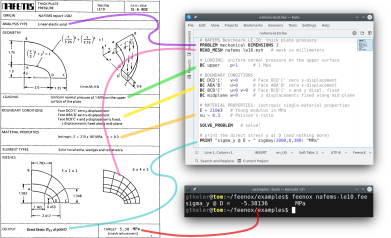
\includegraphics[width=0.95\textwidth,height=\textheight]{nafems-le10-problem-input.svg}
\end{frame}

\begin{frame}[fragile]{NAFEMS LE11: everything is an expression
(especially temperature)}
\protect\hypertarget{nafems-le11-everything-is-an-expression-especially-temperature}{}
\begin{columns}[T]
\begin{column}{0.5\textwidth}
\centering 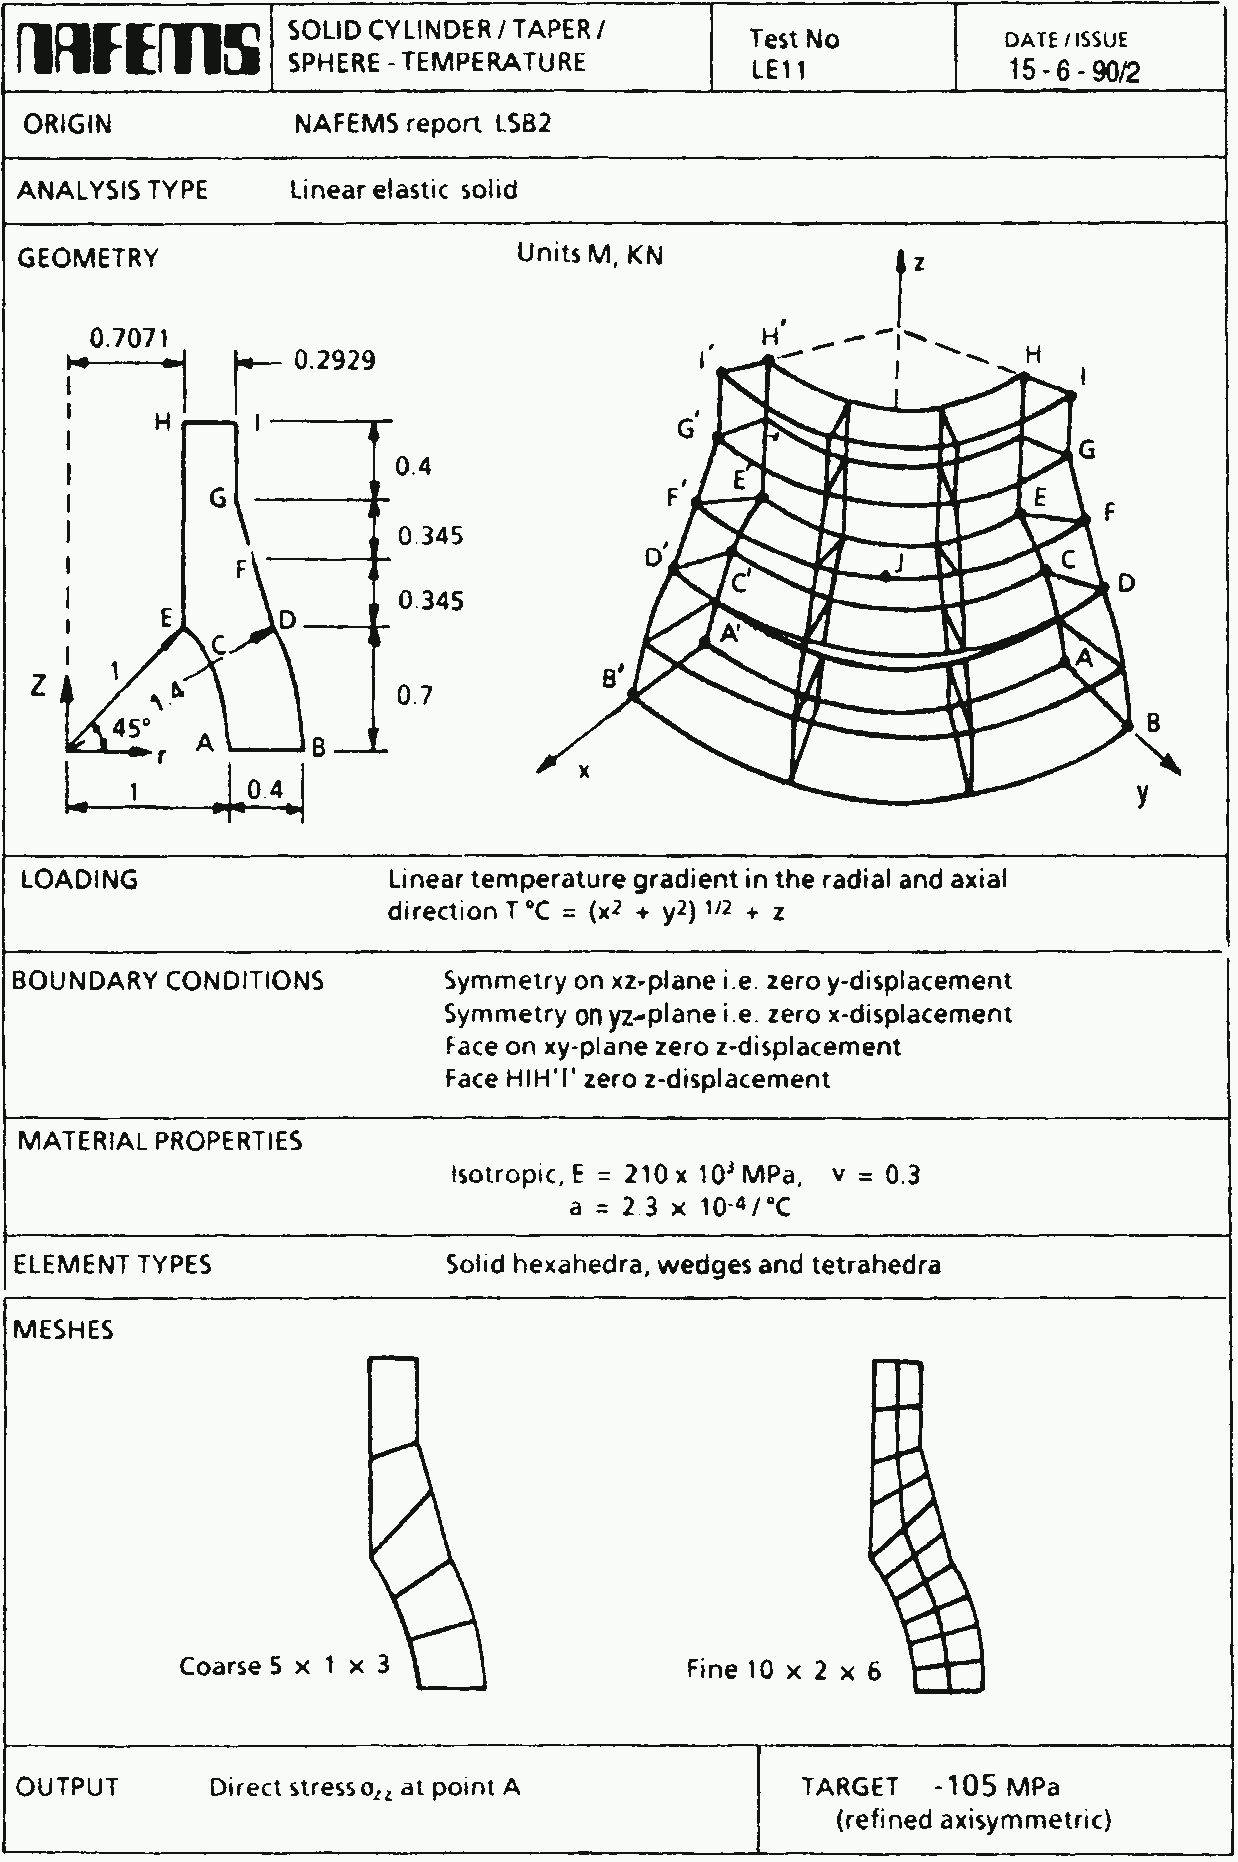
\includegraphics[width=0.75\textwidth,height=\textheight]{nafems-le11.png}
\end{column}

\pause

\begin{column}{0.5\textwidth}
\begin{lstlisting}[style=feenox]
PROBLEM mechanical 3D
READ_MESH nafems-le11.msh

# linear temperature gradient in the radial and axial direction
T(x,y,z) := sqrt(x^2 + y^2) + z  # UTEMP for this????

BC xz     v=0       # displacement vector is [u,v,w]
BC yz     u=0       # u = displacement in x
BC xy     w=0       # v = displacement in y
BC HIH'I' w=0       # w = displacement in z

E = 210e3*1e6       # mesh is in meters, so E=210e3 MPa -> Pa
nu = 0.3            # dimensionless
alpha = 2.3e-4      # in 1/ºC as in the problem
SOLVE_PROBLEM

# for post-processing in Paraview
WRITE_MESH nafems-le11.vtk VECTOR u v w   T sigmax sigmay sigmaz

PRINT "sigma_z(A) = " sigmaz(0,1,0)/1e6 "MPa" SEP " "
\end{lstlisting}

\vspace{-0.25cm}\hfill{\footnotesize\textcolor{cyan}{(Rule of {least surprise})}}

\begin{lstlisting}[style=terminal]
$ gmsh -3 -clscale 0.5 nafems-le11.geo
[...]
Info    : 8326 nodes 1849 elements
Info    : Writing 'nafems-le11.msh'...
$ feenox nafems-le11.fee 
sigma_z(A) =  -105.043 MPa
$
\end{lstlisting}
\end{column}
\end{columns}
\end{frame}

\begin{frame}[fragile]{}
\protect\hypertarget{section-10}{}
\begin{columns}[T]
\begin{column}{0.5\textwidth}
\begin{block}{3.2. Output}
\protect\hypertarget{output}{}
\begin{itemize}
\tightlist
\item
  Clean output expected
\item
  Do not clutter the output with

  \begin{itemize}
  \tightlist
  \item
    ASCII art
  \item
    Notices
  \item
    Explanations
  \item
    Page separators
  \end{itemize}
\item
  Output should interpreted by both

  \begin{itemize}
  \tightlist
  \item
    A human
  \item
    A computer
  \end{itemize}
\item
  Open standards and well-documented formats should be preferred
\end{itemize}
\end{block}
\end{column}

\pause

\begin{column}{0.5\textwidth}
\begin{exampleblock}{FeenoX}
\protect\hypertarget{feenox-8}{}
\begin{itemize}
\tightlist
\item
  {\textcolor{cyan}{Rule of {economy}}}: output is completely defined by
  the user
\item
  {\textcolor{cyan}{Rule of {silence}}}: no
  \passthrough{\lstinline!PRINT!} no output
\item
  ASCII columns

  \begin{itemize}
  \tightlist
  \item
    \passthrough{\lstinline!PRINT!} \&
    \passthrough{\lstinline!PRINT\_FUNCTION!}
  \item
    Gnuplot \& compatible
  \item
    Markdown/LaTeX tables
  \end{itemize}
\item
  Post-processing formats

  \begin{itemize}
  \tightlist
  \item
    \passthrough{\lstinline!.msh!}
  \item
    \passthrough{\lstinline!.vtk!}
  \item
    \passthrough{\lstinline!.vtu!}: \textcolor{Orange}{TO-DO}
  \item
    \passthrough{\lstinline!.hdf5!}: \textcolor{Orange}{TO-DO}
  \item
    \passthrough{\lstinline!.frd!}: \textcolor{Orange}{TO-DO} ?
  \end{itemize}
\item
  Dumping of vectors \& matrices

  \begin{itemize}
  \tightlist
  \item
    ASCII
  \item
    PETSc binary
  \item
    Octave (sparse)
  \end{itemize}
\end{itemize}
\end{exampleblock}
\end{column}
\end{columns}
\end{frame}

\begin{frame}[fragile]{Markdown table: natural oscillation frequencies
of a wire}
\protect\hypertarget{markdown-table-natural-oscillation-frequencies-of-a-wire}{}
\begin{columns}[T]
\begin{column}{0.4\textwidth}
Experimental Physics 101 (2004)

\centering 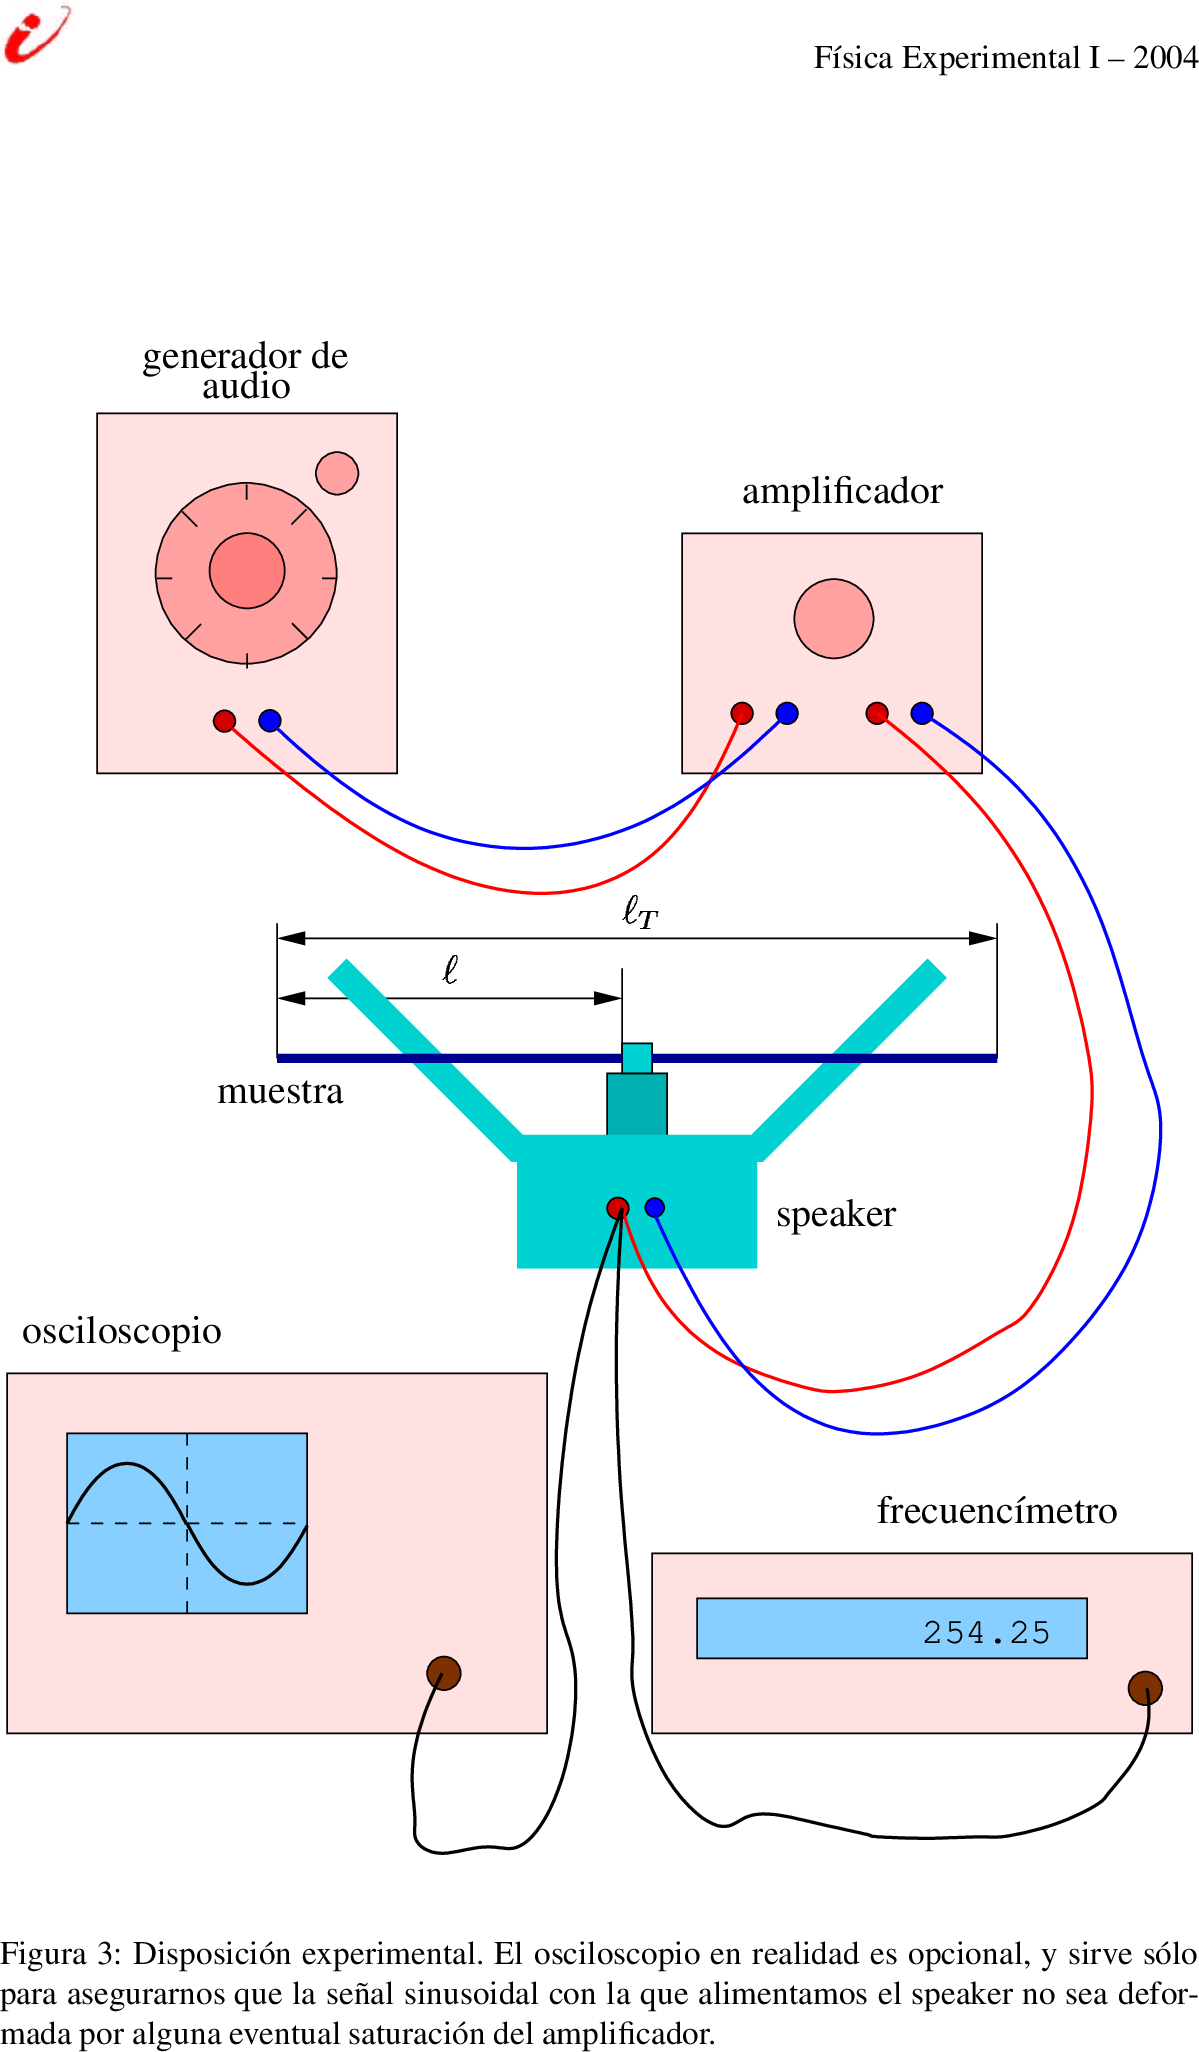
\includegraphics[width=0.7\textwidth,height=\textheight]{wire/alambre-3.png}
\end{column}

\begin{column}{0.6\textwidth}
\begin{lstlisting}[style=feenox]
# compare the frequencies
PRINT "  \$n\$ |   FEM  | Euler | Relative difference [%]"
PRINT ":----:+:------:+:-----:+:-----------------------:"
PRINT_VECTOR i         f(2*i-1) f_euler   100*(f_euler(i)-f(2*i-1))/f_euler(i)
PRINT
PRINT ": $2 wire over $1 mesh, frequencies in Hz"
\end{lstlisting}

\begin{lstlisting}[style=terminal]
$ feenox wire.fee copper hex > copper-hex.md
$
\end{lstlisting}

\begin{longtable}[]{@{}cccc@{}}
\caption{copper wire over hex mesh, frequencies in Hz}\tabularnewline
\toprule()
\(n\) & FEM & Euler & Relative difference {[}\%{]} \\
\midrule()
\endfirsthead
\toprule()
\(n\) & FEM & Euler & Relative difference {[}\%{]} \\
\midrule()
\endhead
1 & 45.8374 & 45.8448 & 0.0161707 \\
2 & 287.126 & 287.302 & 0.0611787 \\
3 & 803.369 & 804.454 & 0.134888 \\
4 & 1572.59 & 1576.41 & 0.242324 \\
5 & 2595.99 & 2605.92 & 0.381107 \\
\bottomrule()
\end{longtable}
\end{column}
\end{columns}
\end{frame}

\begin{frame}{Professional tables: environmentally-assisted fatigue}
\protect\hypertarget{professional-tables-environmentally-assisted-fatigue}{}
\begin{columns}[T]
\begin{column}{0.55\textwidth}
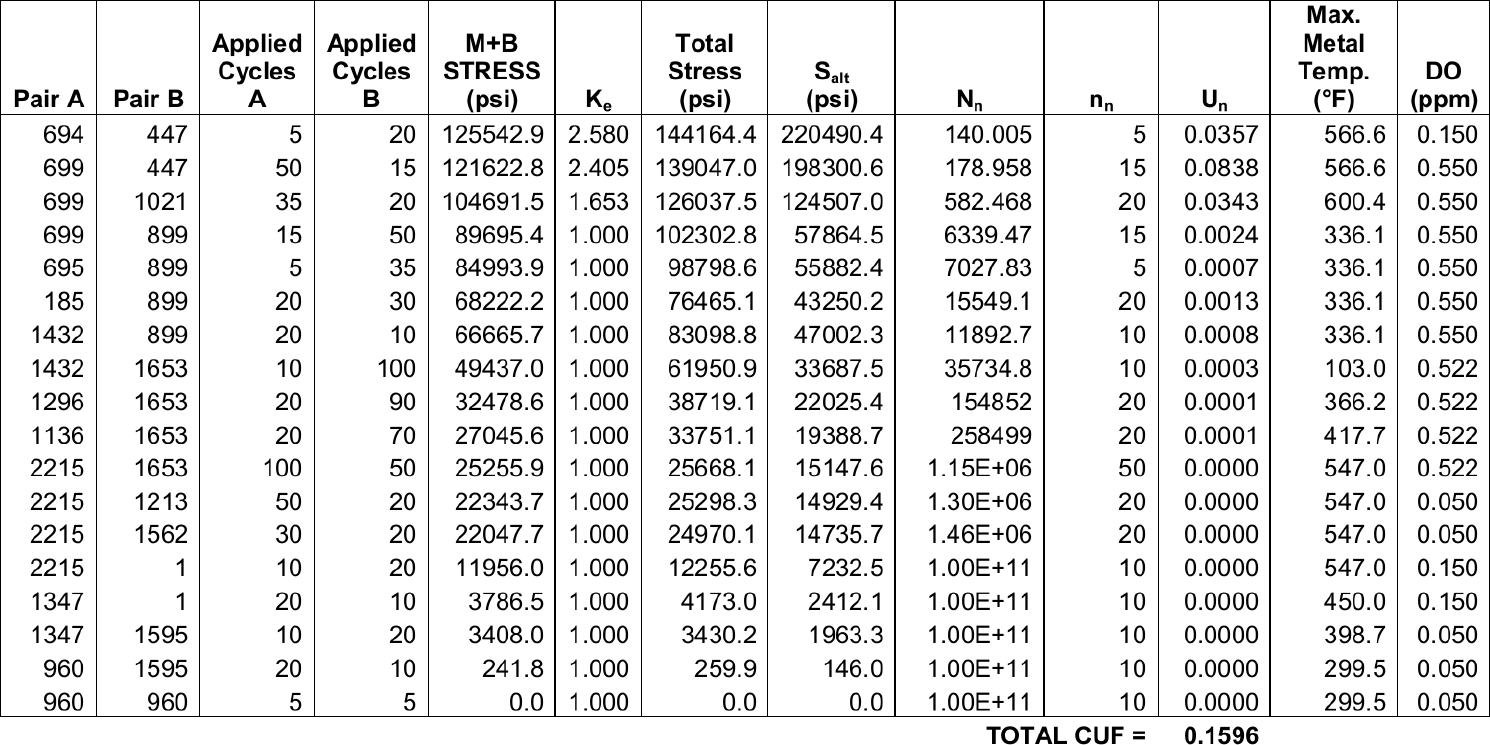
\includegraphics{nureg.png}

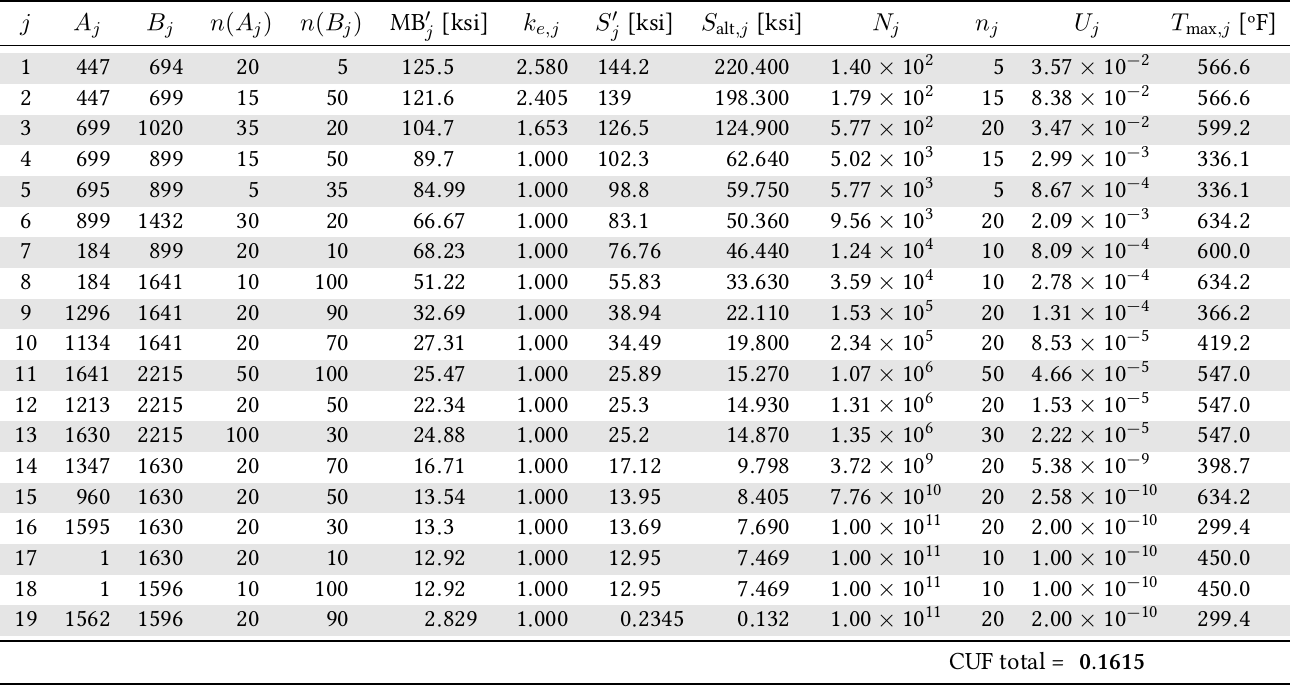
\includegraphics{cne.png}
\end{column}

\begin{column}{0.45\textwidth}
\vspace{1cm}

\begin{itemize}
\tightlist
\item
  Computation of NUREG-EPRI sample problem for Environmentally-assisted
  fatigue in NPP piping
\end{itemize}

\bigskip

\begin{itemize}
\tightlist
\item
  Top is a table from a publication by a multi-billion dollar agency
\item
  Bottom is a PDF from FeenoX output piped through

  \begin{itemize}
  \tightlist
  \item
    AWK
  \item
    \LaTeX
  \end{itemize}
\end{itemize}
\end{column}
\end{columns}
\end{frame}

\begin{frame}[fragile]{}
\protect\hypertarget{section-11}{}
\begin{columns}[T]
\begin{column}{0.5\textwidth}
\begin{block}{4. Quality Assurance}
\protect\hypertarget{quality-assurance}{}
\begin{itemize}
\tightlist
\item
  Generic good software QA practices

  \begin{itemize}
  \tightlist
  \item
    Distributed version control system
  \item
    Automated testing suites
  \item
    User-reported bug tracking support
  \item
    Signed releases
  \item
    etc.
  \end{itemize}
\end{itemize}

\begin{block}{4.1. Reproducibility and traceability}
\protect\hypertarget{reproducibility-and-traceability}{}
\begin{itemize}
\tightlist
\item
  Both the source and the documentation should be tracked with a DVCS
\item
  Repository should be accessible online

  \begin{itemize}
  \tightlist
  \item
    Might need credentials even for RO
  \end{itemize}
\item
  Version reporting

  \begin{itemize}
  \tightlist
  \item
    Executables must allow \passthrough{\lstinline!--version!}
  \item
    Libraries must provide an API call
  \end{itemize}
\item
  The files needed to solve a problem should be simple \& traceable by a
  DVCS
\end{itemize}
\end{block}
\end{block}
\end{column}

\pause

\begin{column}{0.5\textwidth}
\begin{exampleblock}{FeenoX}
\protect\hypertarget{feenox-9}{}
\begin{itemize}
\tightlist
\item
  Hosted on Github (\passthrough{\lstinline!git!})

  \begin{itemize}
  \tightlist
  \item
    Previously on Bitbucket (\passthrough{\lstinline!hg!})
  \item
    Previously on Launchpad (\passthrough{\lstinline!bzr!})
  \item
    Previously on-premise (\passthrough{\lstinline!svn!})
  \end{itemize}
\item
  \url{https://github.com/seamplex/feenox}
\item
  \url{https://seamplex.com/feenox}
\item
  Mailing list (Google group)
\item
  Build a community! \textcolor{Orange}{TO-DO}

  \begin{itemize}
  \tightlist
  \item
    Code of conduct
  \end{itemize}
\end{itemize}

\begin{lstlisting}[style=terminal]
$ feenox
FeenoX v0.1.12-gb9a534f-dirty 
a free no-fee no-X uniX-like finite-element(ish) computational engineering tool

usage: feenox [options] inputfile [replacement arguments]
[...]
$
\end{lstlisting}

\begin{itemize}
\item
  \passthrough{\lstinline!-v!}/\passthrough{\lstinline!--version!}:
  copyright notice
\item
  \passthrough{\lstinline!-V!}/\passthrough{\lstinline!--versions!}:
  linked libraries
\item
  {\textcolor{cyan}{Rule of {generation}}}: inputs from M4
\end{itemize}
\end{exampleblock}
\end{column}
\end{columns}
\end{frame}

\begin{frame}[fragile]{}
\protect\hypertarget{section-12}{}
\begin{columns}[T]
\begin{column}{0.5\textwidth}
\begin{block}{4.2. Automated testing}
\protect\hypertarget{automated-testing}{}
\begin{itemize}
\tightlist
\item
  A mean to test the code is mandatory
\item
  After each change

  \begin{itemize}
  \tightlist
  \item
    Check for regressions
  \item
    Problems with already-computed solutions
  \item
    Different from verification
  \end{itemize}
\item
  The compiler should not issue warnings
\item
  Dynamic memory allocation checks are recommended
\item
  Good practices are suggested

  \begin{itemize}
  \tightlist
  \item
    Unit testing
  \item
    Continuous integration
  \item
    Test coverage analysis
  \end{itemize}
\end{itemize}
\end{block}

\begin{block}{4.3. Bug reporting and tracking}
\protect\hypertarget{bug-reporting-and-tracking}{}
\begin{itemize}
\tightlist
\item
  Users should be able to report bugs

  \begin{itemize}
  \tightlist
  \item
    A task should be created for each report
  \item
    Address and document
  \end{itemize}
\end{itemize}
\end{block}
\end{column}

\pause

\begin{column}{0.5\textwidth}
\begin{exampleblock}{FeenoX}
\protect\hypertarget{feenox-10}{}
\begin{itemize}
\item
  Standard test suite

\begin{lstlisting}[style=terminal]
$ make check
Making check in src
[...]
PASS: tests/trig.sh
PASS: tests/vector.sh
=============================================
Testsuite summary for feenox v0.1.12-gb9a534f
=============================================
# TOTAL: 26
# PASS:  25
# SKIP:  0
# XFAIL: 1
# FAIL:  0
# XPASS: 0
# ERROR: 0
=============================================
$
\end{lstlisting}
\item
  Periodic \passthrough{\lstinline!valgrind!} runs
\item
  Integration tests: \textcolor{Orange}{TO-DO}
\item
  CI \& test coverage: \textcolor{Orange}{TO-DO}
\end{itemize}

\medskip

\begin{itemize}
\tightlist
\item
  Github issue tracker
\item
  Branching \& merging procedures: \textcolor{Orange}{TO-DO}
\end{itemize}
\end{exampleblock}
\end{column}
\end{columns}
\end{frame}

\begin{frame}[fragile]{}
\protect\hypertarget{section-13}{}
\begin{columns}[T]
\begin{column}{0.5\textwidth}
\begin{block}{4.4 Verification}
\protect\hypertarget{verification}{}
\begin{itemize}
\tightlist
\item
  Code must be always verified
\item
  Check it solves \textbf{right the equations}

  \begin{itemize}
  \tightlist
  \item
    MES (mandatory)
  \item
    MMS (recommended)
  \end{itemize}
\item
  One test case has to be added to the automated testing
\item
  Third-party verification should be allowed
\item
  Per-problem documentation
\end{itemize}
\end{block}

\begin{block}{4.5. Validation}
\protect\hypertarget{validation}{}
\begin{itemize}
\tightlist
\item
  Code should be validated as required
\item
  Check it solves \textbf{the right equations}

  \begin{itemize}
  \tightlist
  \item
    Against experiments
  \item
    Against other codes
  \end{itemize}
\item
  Third-party validation should be allowed
\item
  Per-application/industry documentation

  \begin{itemize}
  \tightlist
  \item
    Procedures following standards
  \end{itemize}
\end{itemize}
\end{block}
\end{column}

\pause

\begin{column}{0.5\textwidth}
\begin{exampleblock}{FeenoX}
\protect\hypertarget{feenox-11}{}
\begin{itemize}
\item
  There is a V\&V report for the industrial human-less workflow project

  \begin{itemize}
  \tightlist
  \item
    Medical devices
  \item
    Based on ASME V\&V 40
  \end{itemize}
\item
  There is a lot to do!
\item
  MES

  \begin{itemize}
  \tightlist
  \item
    Set of well-known benchmarks
  \item
    NAFEMS, IAEA, etc.
  \end{itemize}
\item
  MMS

  \begin{itemize}
  \tightlist
  \item
    Everything is an expression
  \item
    Parametric runs
  \item
    \passthrough{\lstinline!MESH\_INTEGRATE!} allows to compute \(L_2\)
    norms directly in the \passthrough{\lstinline!.fee!}
  \end{itemize}
\end{itemize}

\bigskip

\begin{itemize}
\tightlist
\item
  TL;DR: \textcolor{Orange}{TO-DO}
\end{itemize}
\end{exampleblock}
\end{column}
\end{columns}
\end{frame}

\begin{frame}{}
\protect\hypertarget{section-14}{}
\begin{columns}[T]
\begin{column}{0.5\textwidth}
\begin{block}{4.6. Documentation}
\protect\hypertarget{documentation}{}
\begin{itemize}
\tightlist
\item
  Documentation should be complete

  \begin{itemize}
  \tightlist
  \item
    User manual

    \begin{itemize}
    \tightlist
    \item
      Tutorial
    \item
      Reference
    \end{itemize}
  \item
    Developer guide
  \end{itemize}
\item
  Quick reference cards, video tutorials, etc. not mandatory but
  recommended
\item
  Non-trivial mathematics and methods

  \begin{itemize}
  \tightlist
  \item
    Explained
  \item
    Documented
  \end{itemize}
\item
  Should be available as hard copies and mobile-friendly online
\item
  Clear licensing scheme for the documentation

  \begin{itemize}
  \tightlist
  \item
    People extending the functionality ought to be able to document
    their work
  \end{itemize}
\end{itemize}
\end{block}
\end{column}

\begin{column}{0.5\textwidth}
\begin{exampleblock}{FeenoX}
\protect\hypertarget{feenox-12}{}
\begin{itemize}
\tightlist
\item
  FeenoX is not compact!

  \begin{itemize}
  \tightlist
  \item
    Even I have to check the reference
  \end{itemize}
\item
  Commented sources: \textcolor{Plum}{TO-DO}

  \begin{itemize}
  \tightlist
  \item
    Keywords
  \item
    Functions
  \item
    Functionals
  \item
    Variables
  \item
    Material properties
  \item
    Boundary conditions
  \item
    Solutions
  \end{itemize}
\item
  Shape functions: \textcolor{Plum}{TO-DO}
\item
  Gradient recovery: \textcolor{Plum}{TO-DO}
\item
  Mathematical models: \textcolor{Plum}{TO-DO}
\end{itemize}

\medskip

\begin{itemize}
\tightlist
\item
  Code is GPLv3+
\item
  Documentation is GFDLv1.3+
\end{itemize}
\end{exampleblock}
\end{column}
\end{columns}
\end{frame}

\begin{frame}{Conclusions---FeenoX\ldots{}}
\protect\hypertarget{conclusionsfeenox}{}
\begin{itemize}
\tightlist
\item
  is to FEA what Markdown is to documentation
\item
  is (so far) the only tool that fulfills 100\% a fictitious SRS:

  \begin{itemize}
  \tightlist
  \item
    Free and open source (GPLv3+)
  \item
    No recompilation needed
  \item
    Cloud-first and web friendly
  \item
    Human-less workflow
  \end{itemize}
\item
  follows the {\textcolor{cyan}{UNIX}} philosophy: ``do one thing well''
\end{itemize}
\end{frame}

\end{document}
